\documentclass[oneside,12pt]{Classes/uitBA}
  \university{{HANOI UNIVERSITY OF SCIENCE AND TECHNOLOGY}}
  \collegeordept{{SCHOOL OF INFORMATION AND COMMUNICATION TECHNOLOGY}}
    %\crest{
\includegraphics[scale=.30]{HUST}} 
  \mydegree{ENGINEER}  
  \title{STRUCTURED LIGHT USING DE BRUIJN SEQUENCE FOR RANGE DATA ACQUISITION} 
    \author{{Nguyen Thanh Trung}}   
  \degreedate{08-2016} 
\hbadness=10000
\hfuzz=50pt
\usepackage{StyleFiles/watermark}
\onehalfspacing
\hypersetup{colorlinks = false}
\usepackage{gensymb}
\usepackage[justification=centering,font=small,labelfont=bf]{caption} 
\usepackage[ruled,vlined]{algorithm2e}
\SetAlFnt{\footnotesize}
\SetKw{KwDownTo}{downto}
\SetKw{KwTrue}{true}
\SetKw{KwFalse}{false}
\SetKw{KwContinue}{continue}
\SetKw{KwBreak}{break}
\SetKwInOut{Input}{Input}
\SetKwInOut{Output}{Output}
\SetKw{KwAnd}{and}
\SetKw{KwOr}{or}
\makeatletter
\newcommand{\nosemic}{\renewcommand{\@endalgocfline}{\relax}}% Drop semi-colon ;
\makeatother

\usepackage[outdir=./]{epstopdf}
\usepackage{amsthm}
\newtheorem{mydef}{Definition}
\usepackage{listings}
\lstset{ %
  basicstyle=\ttfamily\footnotesize,        % the size of the fonts that are used for the code
  breakatwhitespace=false,         % sets if automatic breaks should only happen at whitespace
  breaklines=true,                 % sets automatic line breaking
  captionpos=b,                    % sets the caption-position to bottom
  keepspaces=true,                 % keeps spaces in text, useful for keeping indentation of code (possibly needs columns=flexible)
  numbers=left,                    % where to put the line-numbers; possible values are (none, left, right)
  numbersep=5pt,                   % how far the line-numbers are from the code
  tabsize=2,	                   % sets default tabsize to 2 spaces
  title=\lstname                   % show the filename of files included with \lstinputlisting; also try caption instead of title
}


\begin{document}
\maketitle
\setcounter{secnumdepth}{3}
\setcounter{tocdepth}{3}

\frontmatter % book mode only
\pagenumbering{roman}
\begin{acknowledgements}      

Though only my name appears on the cover of this thesis, a great many people have contributed to its production. I owe my gratitude to all those people who have made this thesis possible and because of whom my graduate experience has been one that I will cherish forever.
My deepest gratitude is to my supervisor, Prof. Nguyen Khanh Van. I have been amazingly fortunate to have an supervisor who gave me the freedom to explore on my own, and at the same time the guidance to recover when my steps faltered. He taught me how to question thoughts and express ideas.

Mrs. Nguyen Phi Le's insightful comments and constructive criticisms at different stages of my research were thought-provoking and they helped me focus my ideas. I am also thankful to her for reading my reports, commenting on my views and helping me understand and enrich my ideas.

I am also indebted to the members of SEDIC Lab with whom I have interacted during the course of my studies. Particularly, I would like to acknowledge Mr. Nguyen Duc Trong, Mr. Truong Thao Nguyen for the many valuable discussions that helped me understand my research area better.

I am also grateful to the current lecturers at School of Information and Communication Technology, for their various forms of support during my college study.

Many friends have helped me stay sane through these difficult years -- Đô, Lù, and Na and especially \#Reiju Vinsmoke. Their support and care helped me overcome setbacks and stay focused on my study. Thank you for giving me hope and bringing light to my life.

Most importantly, none of this would have been possible without the love and patience of my family. My immediate family to whom this thesis is dedicated to, has been a constant source of love, concern, support and strength all these years. I would like to express my heart-felt gratitude to my family.

\end{acknowledgements}
  
\begin{acknowledgementslong}      
\textbf{1. Student information}

Student name: Nguyen Thanh Trung

\begin{tabular}{@{}l l l l}
Tel: & 0977366197 & Email: & 20102380@student.hut.edu.vn \\ 
Class: & IS-K56 & Program:  & HEDSPI
\end{tabular}

This thesis is performed at: Hanoi University of Science and Technology \\
From 05/09/2015 to 27/05/2016

\textbf{2. Goals of thesis}

\begin{itemize}
\item Study related works about Geographical routing in Wireless Sensor Network with holes
\item Propose a hole bypassing routing scheme for the near hole routing problem ensuring both requirements: energy efficiency and load balancing
\end{itemize}

\textbf{3. Main tasks}
\begin{itemize}
\item Study related works about Geographical routing in Wireless Sensor Network with holes
\item Propose a hole bypassing routing scheme for the near hole routing problem ensuring both requirements: energy efficiency and load balancing
\item Modify the BK-WisSim toolkit to adapt more requirements of network simulation
\item Implement proposed protocol and do experimental evaluations to compare it with current protocols
\end{itemize}


\textbf{4. Declaration of student}

I – Nguyen Thanh Trung - hereby warrants that the Work and Presentation in this thesis are performed by myself under the supervision of Assoc. Prof. Yamaguchi Masahiro.

All results presented in this thesis are truthful and are not copied from any other work.

\begin{tabular}{l l l c }
    \textbf{ } \hspace*{35pt} \textbf{ } &  \textbf{ } \hspace*{35pt} \textbf{ } & \textbf{ } \hspace*{35pt} \textbf{ } & Hanoi, 27/05/2016 \\ 
    \textbf{ } \hspace*{35pt} \textbf{ } &  \textbf{ } \hspace*{35pt} \textbf{ } & \textbf{ } \hspace*{35pt} \textbf{ } & Author \\
    \\
    \\
    \\
    \textbf{ } \hspace*{35pt} \textbf{ } &  \textbf{ } \hspace*{35pt} \textbf{ } & \textbf{ } \hspace*{35pt} \textbf{ } & Vu Quoc Huy
    \end{tabular}

    
\textbf{5. Attestation of the supervisor on the fulfillment of the requirements of the thesis}
\\[5cm]
\begin{tabular}{l l l c }
    \textbf{ } \hspace*{35pt} \textbf{ } &  \textbf{ } \hspace*{35pt} \textbf{ } & \textbf{ } \hspace*{35pt} \textbf{ } & Hanoi, 27/05/2016 \\ 
    \textbf{ } \hspace*{35pt} \textbf{ } &  \textbf{ } \hspace*{35pt} \textbf{ } & \textbf{ } \hspace*{35pt} \textbf{ } & Supervisor \\
    \\
    \\
    \\
    \textbf{ } \hspace*{35pt} \textbf{ } &  \textbf{ } \hspace*{35pt} \textbf{ } & \textbf{ } \hspace*{35pt} \textbf{ } & Prof. Yamaguchi Masahiro
    \end{tabular}

\end{acknowledgementslong}
  
\begin{abstracts}         
Một vấn đề quan trọng trong nghiên cứu xây dựng các thuật toán định tuyến cho mạng cảm biến không dây là giải quyết bài toán định tuyến trong mạng có hố. Các hố này có thể được sinh ra bởi một vài lý do, bao gồm do trong môi trường có các vật cản tự nhiên dẫn đến không thể triển khai, hoặc do các thảm họa tự nhiên gây nên. Do đó hình dạng hố rất ngẫu nhiên, có thể là các hình đa giác lõm phức tạp. Một số thuật toán đã được đưa ra để giải quyết bài toán định tuyến với hố bằng việc định nghĩa một vùng cấm quanh hố, kết hợp với một số yếu tố ngẫu nhiên qua đó giúp mạng cân bằng tải và tiêu thụ năng lượng tốt hơn. Tuy nhiên, đối với bài toán định tuyến gần hố, tức là bài toán tìm đường định tuyến có nguồn hoặc đích nằm trong các vùng cấm, các nghiên cứu này đều chưa đưa ra được một thuật toán định tuyến hiệu quả, mà chủ yếu dựa vào thuật toán định tuyến tham lam. Trong đồ án này, chúng tôi đề xuất một thuật toán định tuyến giải quyết bài toán định tuyến gần hố, sử dụng sơ đồ Voronoi để xây dựng lên các đường định tuyến “thoát hố”. Kết quả thực nghiệm cho thấy giải pháp đề xuất có kết quả tốt hơn các thuật toán định tuyến tham lam và thuật toán BOUNDHOLE trên các phương diện: năng lượng, cân bằng tải, độ dài đường định tuyến. 
\end{abstracts}
 
\begin{abstractsEnglish}         
Geographic routing is well suited for large-scale wireless sensor networks (WSNs) since it is nearly stateless. It can achieve a near-optimal routing path in the networks without of holes because of its simplicity and scalability. With the occurrence of holes, however, geographic routing faces the problems of hole diffusion and routing path enlargement. The hole shape could be very complex with many cave regions. Several recent proposals attempt to fix these issues by deploying a special, forbidding area around the hole, which helps to improve the congestion on the hole boundary but still are deficient since they use the perimeter routing scheme to bypass the hole within the forbidden area. In this thesis, we introduce a novel approach which is the first to target and solve the near hole routing problem, while ensuring both two requirements: energy consumption and load balancing. Our simulation experiments show that our scheme strongly outperforms the existing schemes in several performance factors, including route stretch, efficient use of energy and load balancing.
\end{abstractsEnglish}
 
\tableofcontents
\listoffigures
  %\addcontentsline{toc}{chapter}{Nomenclature}

\mainmatter
% \part{Introduction}
\chapter{Introduction}
\section{Overview}
\subsection{Wireless Sensor Network Overview}
Recent advances in micro-electro-mechanical systems, embedded processors, and wireless communications have led to the emergence of Wireless sensor networks (WSNs) \cite{wsn-survey}, which consist of a large number of sensing devices each capable of sensing, processing and transmitting environmental information. Applications of wireless sensor network include battlefield surveillance \cite{wsn-app}, biological detection, smart spaces \cite{wsn-app}, industrial diagnostics, and so on. Another important application of wireless sensor network that cannot be left out is environmental monitoring, analyzing and forecasting disasters such as Forest fire detection, Flood detection, ... We envision that, in near future, wireless sensor networks will be more popular and be an integral part of our lives.

One of the most important constraints on sensor nodes is the low power consumption requirement. The wireless sensor node can only be equipped with a limited, generally irreplaceable, power source. Therefore, while traditional networks aim to achieve high quality of service (QoS), sensor network protocols must focus primarily on power conservation. In an ad hoc sensor network, each node plays the dual role of data originator and data router. The dis-functioning of few nodes can cause significant topological changes and might require re-routing of packets. Hence, power conservation and power management take on additional importance.

Another essential property of wireless sensor networks is its scalability and distribution. The number of sensor nodes deployed in studying a phenomenon may be in the order of hundreds or thousands. Depending on the application, the number may reach an extreme value of millions, for instance, the forest fire detection system may contain thousands sensor nodes.

In the wireless sensor network, communicating nodes are linked by a wireless medium. Thus, a sensor node can only communicate with sensor nodes which lie within its communication range. In case of communicating two sensor nodes which do not lie within each other's communication range, the packet have to be transmitted via intermediate nodes. The routing path of packets is calculated depending on the routing protocol that network uses.


\subsection{Geographical routing in Wireless Sensor Network}
Routing protocols in wireless sensor network recently has attracted much concerns from researchers. The designing of routing protocols in wireless sensor network is challenging due to its mentioned properties. For example, in the traditional network such as Ethernet, a node can analysis whole network to find out the optimal routing path, however, it is impossible to do this task in wireless sensor network. The requirements of routing protocols in wireless sensor network not only includes low latency, fault tolerance, but also has to guarantee following factors:

\begin{itemize}
\item \emph{Computational complexity}: sensor nodes have very limited and low hardware power so the complexity of the algorithm has to be as simple as possible. For example, the wide use sensor node, Mica 2 Mote \cite{mica2}, has only 128K bytes of program flash memory and uses a 8-bit micro-controller.
\item \emph{Energy consumption}: because of limited and irreplaceable power source, the routing protocol has to be energy efficiency.
\item \emph{Load balancing}: the load balance has a big impact on the energy consumption of sensor nodes. Network congestion causes some sensor nodes carry more data than the others and quickly die. Consequently, it significantly changes the connectivity and topology of the network. Thus, load balancing plays an important role in routing in wireless sensor networks.
\end{itemize} 

A common approach is using geographical location information of sensor nodes to design the routing protocols. It is well suited for large-scale wireless sensor networks because it is nearly stateless. The class of these protocols is named \emph{geographical routing protocols}. This approach assumes that exact location of sensor nodes is known beforehand. In other words, the routing path of the packet is conducted from the geographical location information of sensor nodes. Notice that, in geographical routing, each sensor node only needs to know its neighbors' location information (a 1-hop neighbor of a sensor node \emph{S} is a node which is inside the communication range of \emph{S}). When a sensor node receives a packet, it decides to forward this packet to one of its neighbors based on current location information of its neighbors. 

A classical algorithm in this type of protocols is the greedy algorithm \cite{wsn-greedy}. The greedy algorithm is described as follows: the packet is forwarded to a neighbor which is closer to the destination node than current node and closest to the destination node among all neighbor nodes. Greedy forwarding’s great advantage is its reliance only on knowledge of the forwarding node’s immediate neighbors. The state required is negligible, and dependent on the density of nodes in the wireless network, not the total number of destinations in the network. However, the biggest problem of greedy algorithm is the occurrence of the local minimum phenomenon, i.e. there is no satisfying neighbor to forward the packet anymore. Figure \ref{local-minimum} demonstrates this phenomenon. This problems is usually caused by the existence of \emph{routing holes} in the network topology.
\begin{figure}[!htb]
\centering
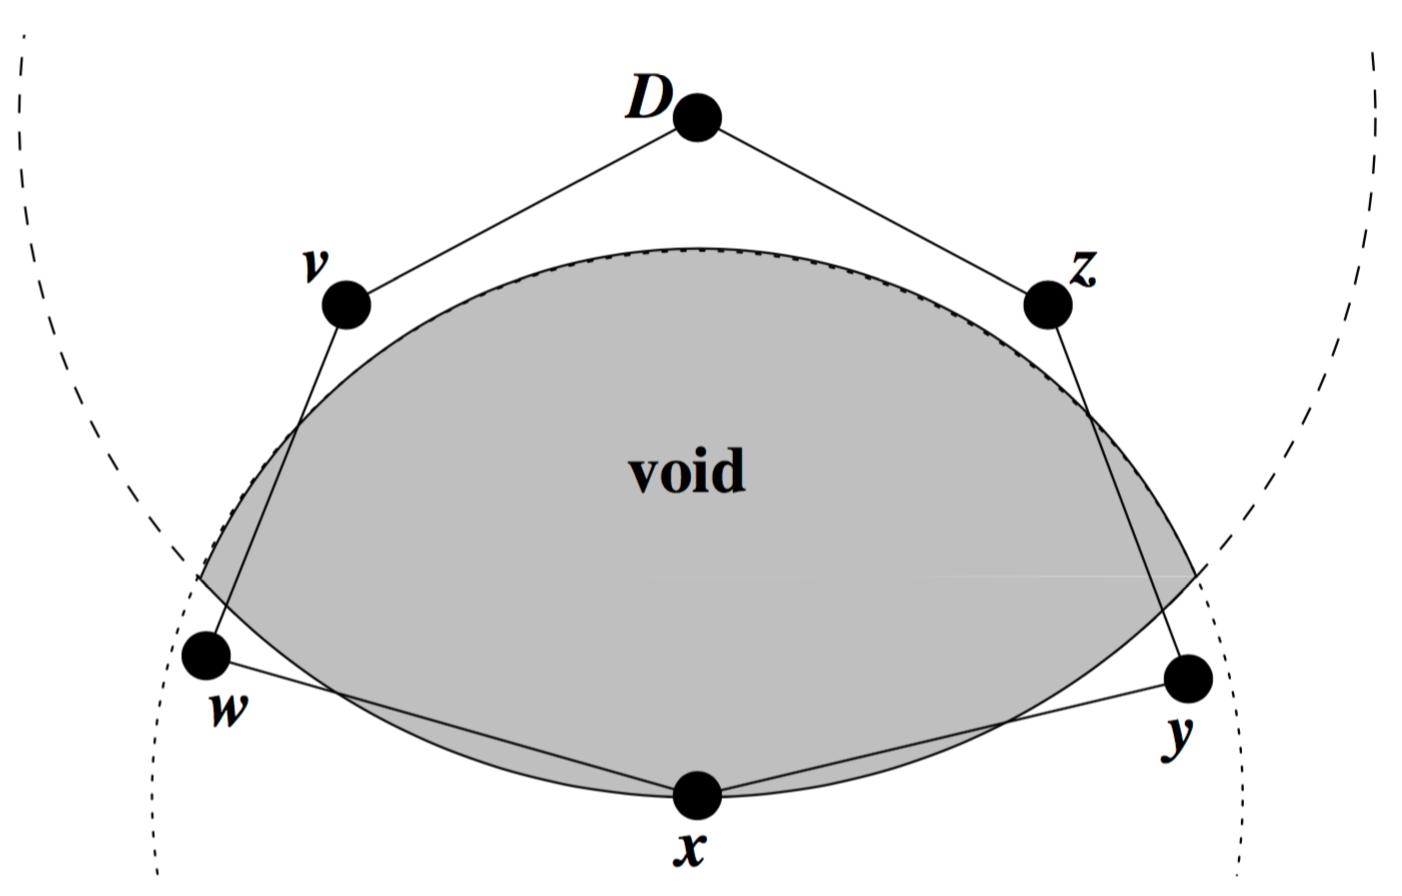
\includegraphics[width=0.4\textwidth]{Chapter1/Chapter1Figs/fig-local-minimum.png}
\caption{Node $x$’s void with respect to destination $D$.}
\label{local-minimum}
\end{figure}

A \emph{routing hole} in a wireless sensor network is a region where either there are no sensor nodes or the available nodes cannot participate in the activity of the network, i.e. they cannot communicate with the rest of the network. These holes can be formed either due to voids in sensor deployment or because of failure of sensor nodes due to various reasons such as malfunctioning, battery depletion or an external event such as fire, flood or structure collapse physically destroying the nodes. The local minimum phenomenon likely occurs when a routing hole is encountered. In the next chapter, we will discuss several previous works attempting to detect routing holes and to route the packet around them in greedy forwarding.

% \chapter{Objectives}
\section{Thesis statement}
\subsection{Thesis statement}\label{thesis-statement}
Several solutions has been proposed to deal with the routing problem in wireless sensor network with holes \cite{gpsr,boundhole,ehds,elbar,ellipse,issnip}. The most well-known solution is the Greedy Perimeter Stateless Routing (\emph{GPSR}) protocol, which was proposed by B.Karp in 2000 \cite{gpsr}. This algorithm computes a planar graph for the network in which its vertices are sensor nodes and its edges are edges connecting sensor nodes and its neighbors. The packet is then forwarded based on edges of the graph. In 2005, Qing Fang and her colleagues proposed a novel algorithm (the BOUNDHOLE algorithm) to detect the boundary of the routing hole \cite{boundhole}. In addition, these authors also proposed a routing protocol based on the determined hole boundary: when the packet reaches a \emph{stuck node}\footnote{A stuck node is a node where a packet may get stuck and is more likely to occur the local minimum phenomenon. We will discuss further more about stuck node definition in section \ref{chapter3.1-boundhole}.} \emph{S}, it is forwarded along the boundary of the hole until it reaches an intermediate sensor node that is closer to the destination node than \emph{S}. 

Other solutions based on the BOUNDHOLE algorithm has also been proposed. The common idea is that these protocols construct a forbidden area covering the hole and broadcast the information of this area to the network. The source node then uses these information to calculate the routing path. The forbidden area is usually a simpler shape such as circle \cite{ehds}, ellipse \cite{ellipse}, parallelogram \cite{elbar}, or octagon \cite{issnip}. In \cite{issnip}, the authors also proposed a non-trivial approach that is to use some random factors to ensure mentioned requirements of routing in wireless sensor network such as load balancing, energy efficiency and route stretch.

\begin{figure}[!htb]
\centering
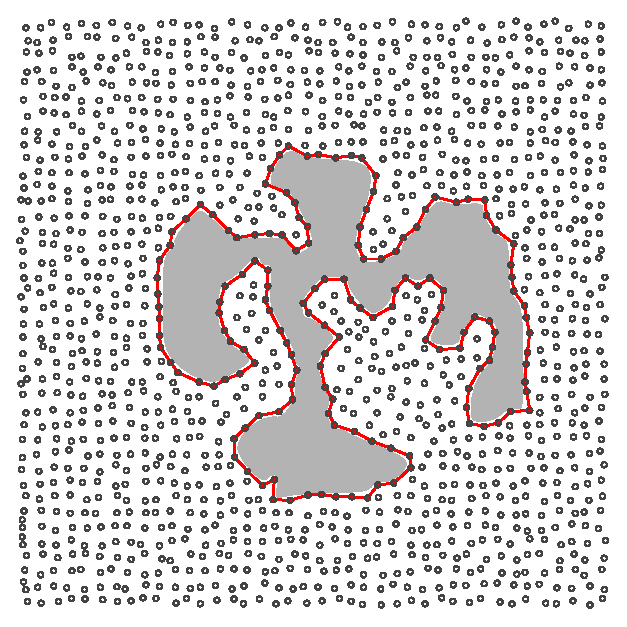
\includegraphics[width=0.4\textwidth]{Chapter2/Chapter2Figs/fig-polygon.eps}
\caption{An example of hole polygon.}
\centering
\small {In this figure, the gray region is the hole and the red line is the hole boundary.}
\label{cave-regions}
\end{figure}

However, the routing hole in wireless sensor network can be a random, complex shape and thus, may have a lot of cave regions. Figure \ref{cave-regions} shows an example of hole shape. \emph{Near hole routing} problem is defined as a problem to find the routing path in which the source node or the destination node, or both of them lie nearly the hole, in the boundary of the hole or inside the cave areas. The difficulty of this problem probably is to construct a path for packet to route out the hole when the source node is inside a cave or to construct a path to forward packet from outside to a destination which is inside a cave. Most of the above algorithms have been ignored the near hole routing problem. In such a case, they all use the GPSR algorithm to compute the routing path. This generally degrades the efficiency of these protocols in case there requires a lot of near hole routings. This leads to the necessity of a good \emph{near hole routing protocol} to fulfill requirements of routing in wireless sensor networks.

\subsection{Objectives}
Based on the described problem in subsection \ref{thesis-statement}, the objectives of my thesis are:
\begin{enumerate}
\item \emph{Study related works about geographical routing in wireless sensor network with holes.} We need to make a survey about previous works: their advantages and disadvantages. Generally, a routing protocol consists of two phases: the initial phase when the network learns about the hole shape and computes parameters of the protocol and the data forwarding phase when the network starts sending data packets. Most of previous works use different shapes to approximate the hole polygon in the initial phase. Thus, it is supposed to analyze these shapes to find out the most appropriate shape for the hole approximation since the approximate hole impacts the load balancing, routing stretch and hence, network's energy consumption.
\item \emph{Propose a solution for the near hole routing problem.} Currently, as our knowledge, there are no protocols that can deal with the near hole routing problem except GPSR and BOUNDHOLE. We will propose a protocol which targets to achieve both two main requirements of routing in wireless sensor network with holes, that is load balancing and energy consumption. This is also the main objective of my thesis.
\item \emph{Modify the BK-WisSim toolkit to adapt more requirements of network simulation.} \emph{BK-WisSim} is a visual network simulation tool developed by SEDIC Lab \cite{wissim-web}. We continue developing this tool to support more requirements of network simulation, such as improving the current Energy Model of \emph{ns-2} and developing new features for \emph{BK-WisSim}.
\item \emph{Implement proposed protocol and do experimental evaluations to compare it with current protocols.} The last mission is implementing proposed protocol and embedding it into the core of \emph{BK-WisSim}. Then the proposed protocol will be compared with current exist protocols (GPSR, BOUNDHOLE) to evaluate its performance and proof that it totally satisfies the requirements.
\end{enumerate}

\subsection{Results and Contributions}
\paragraph{Studied related works about geographical routing in wireless sensor network with holes. \\}
We have provided a survey about previous works. In this survey, firstly, we described the BOUNDHOLE algorithm and explained the reason why we need to use this algorithm to detect the routing hole instead of other algorithms; secondly, we described an overview about each protocol and pointed out their pros and cons. We have also come up a conclusion that octagon is the most appropriate shape to use to approximate the hole based on theoretical analyses given by its authors.

\paragraph{Proposed the near hole routing protocol.\\}
This algorithm is my primary research, conducted from studies and research to find a solution for near hole routing problem. This algorithm solves the difficulty of the near hole routing problem by constructing the Voronoi diagram \cite{voronoi} of the hole polygon and then creating a graph which is a \emph{``skeleton''} of this polygon based on the Voronoi diagram. This graph is used to make the routing path for the packet to get out or get in the cave. It also inherits the previous result, that is using octagon to approximate the hole in initial phase and using random factors in routing phase. We also provided some theoretical analyses to prove the validity of the protocol, a discussion about the impact of protocol's parameters. This proposed algorithm not only inherits the advantages of previous algorithm but also completely solves the near hole routing problem.

\paragraph{Updated BK-WisSim toolkit.\\}
We have improved the Energy Model of \emph{ns-2} to support more experimental scenarios and to extract more information about the simulation process. We also developed some new feature for \emph{BK-WisSim} client including: supporting graph algorithms (Voronoi diagram and Dijsktra algorithm) in WisSim Editor, simulating the simulation process via animation in WisSim Visualizer and more. 

\paragraph{Evaluation of proposed protocol.\\}
We proposed some evaluation metrics and scenarios for experiments. These metrics are: energy consumption, deviation of energy consumption, load balancing, routing path length and network lifetime. The experiments were performed to compare the proposed protocol with GPSR and BOUNDHOLE algorithm. The results shown that our proposed protocol is better than both the other algorithms in all evaluation metrics. We also performed some specific experiments for our proposed protocol to analyze the impact of protocol's parameters on energy consumption and routing stretch.

The remainder of this thesis is organized as follows. In chapter \ref{chapter3}, we discuss about the BOUNDHOLE algorithm and related works. The details of proposed protocol is presented in chapter \ref{chapter4}. In this chapter, we firstly describe the protocol details and then provide some theoretical analysis of proposed protocol. In chapter \ref{chapter5}, we give an overview about \emph{ns-2} and \emph{BK-WisSim} toolkit. We also introduce new features of \emph{BK-WisSim} in this chapter. The source code and detailed implementation of proposed protocol is provided in chapter \ref{chapter6}. In chapter \ref{chapter7}, we present the simulation result to evaluate the performance of the protocol. Finally, we conclude the thesis in chapter \ref{chapter8}. 
% \part{Implementation}
\chapter{Routing protocols in Wireless Sensor Network with Holes}\label{chapter3}
We noted that the existence of routing holes in network's topology usually causes the local minimum phenomenon. Thus, a routing protocol has only two options in this scenario, either to drop the packet or to solve the routing hole problem, by using a certain mechanism. There are different methods of dealing with this problem. These protocols have helped us to further define some aspects of our design for the near hole routing protocol. In this chapter, we present these works, and point out their advantages that have been derived in our proposed protocol. 

To approximate the hole polygon, firstly, we have to detect the hole boundary, or, those nodes that lie on the boundary of the hole. This problem is known as the hole boundary detection problem. The detection of hole boundary is important for improving wireless sensor networks operations. 

There is an intuitive way to detect a routing hole. Given a network presented as a Cartesian coordinate system in which each sensor node is a point in the plane, we construct Delaunay triangulation of this network, then with a pre-defined threshold $\eta$, we remove all edges whose length is greater than $\eta$. Remaining edges create some polygons which have more than 3 edges. These polygons may be routing holes. However, the problem of this algorithm is that it is not a distributed protocol, since it requires a central node that has location information of all sensor nodes in the network. Hence, applying this algorithm in case of wireless sensor network may not be effective. Some distributed version of Delaunay triangulation have been proposed, but according to our current knowledge, there is still no truly distributed algorithm.

In 2004, Q.Fang proposed a novel algorithm called \emph{BOUNDHOLE} to detect the hole boundary in a distributed manner. Many routing protocols have adopted the \emph{BOUNDHOLE} algorithm for their hole boundary detection phase. In this chapter, before going into detail of current proposed routing protocols, we will give an overview of \emph{BOUNDHOLE} algorithm.
\section{The TENT rule and BOUNDHOLE algorithm} \label{chapter3.1-boundhole}
\subsection{The TENT rule}
The \emph{TENT rule} is used locally by each sensor node, that is, a node $p$ needs only its 1-hop neighbors and itself location information to determine whether it lies on the boundary of a routing hole. We exemplify the \emph{TENT rule} using representation in figure \ref{tent-rule}. At each node $p$, its neighbors are sorted angularly. For every pair of neighbors $u$ and $v$, where $\overrightarrow{pu}$ is left of $\overrightarrow{pv}$, we consider the perpendicular bisectors of each link (labeled $l1$ and $l2$ in figure \ref{tent-rule}). If the intersection of the bisectors falls outside of the range of $p$, then $p$ has no neighbors closer to the region bounded by the communication range and the bisectors (i.e., the black region in figure \ref{tent-rule}). $p$ is called \emph{``stuck node''} and $\angle upv$ is called \emph{``stuck angle''}. Note that this method locates regions, rather than nodes, where no neighbors are closer. Every node must evaluate its 1-hop neighbors using the \emph{TENT rule}, and only at nodes that the \emph{TENT rule} fails may packets get stuck. If a node $p$ has at least 1 stuck angle, $p$ has to be on the hole boundary. 

This rule also elicits that if angle $upv$ is less than $120\degree$, then there is no stuck angle of $p$ corresponding with pair $(u,v)$. Thus, a sensor node has at most 3 stuck angles.

Upon detecting a failure, stuck nodes are responsible for initiating the \emph{BOUNDHOLE} algorithm.

\begin{figure}[!htb]
\centering
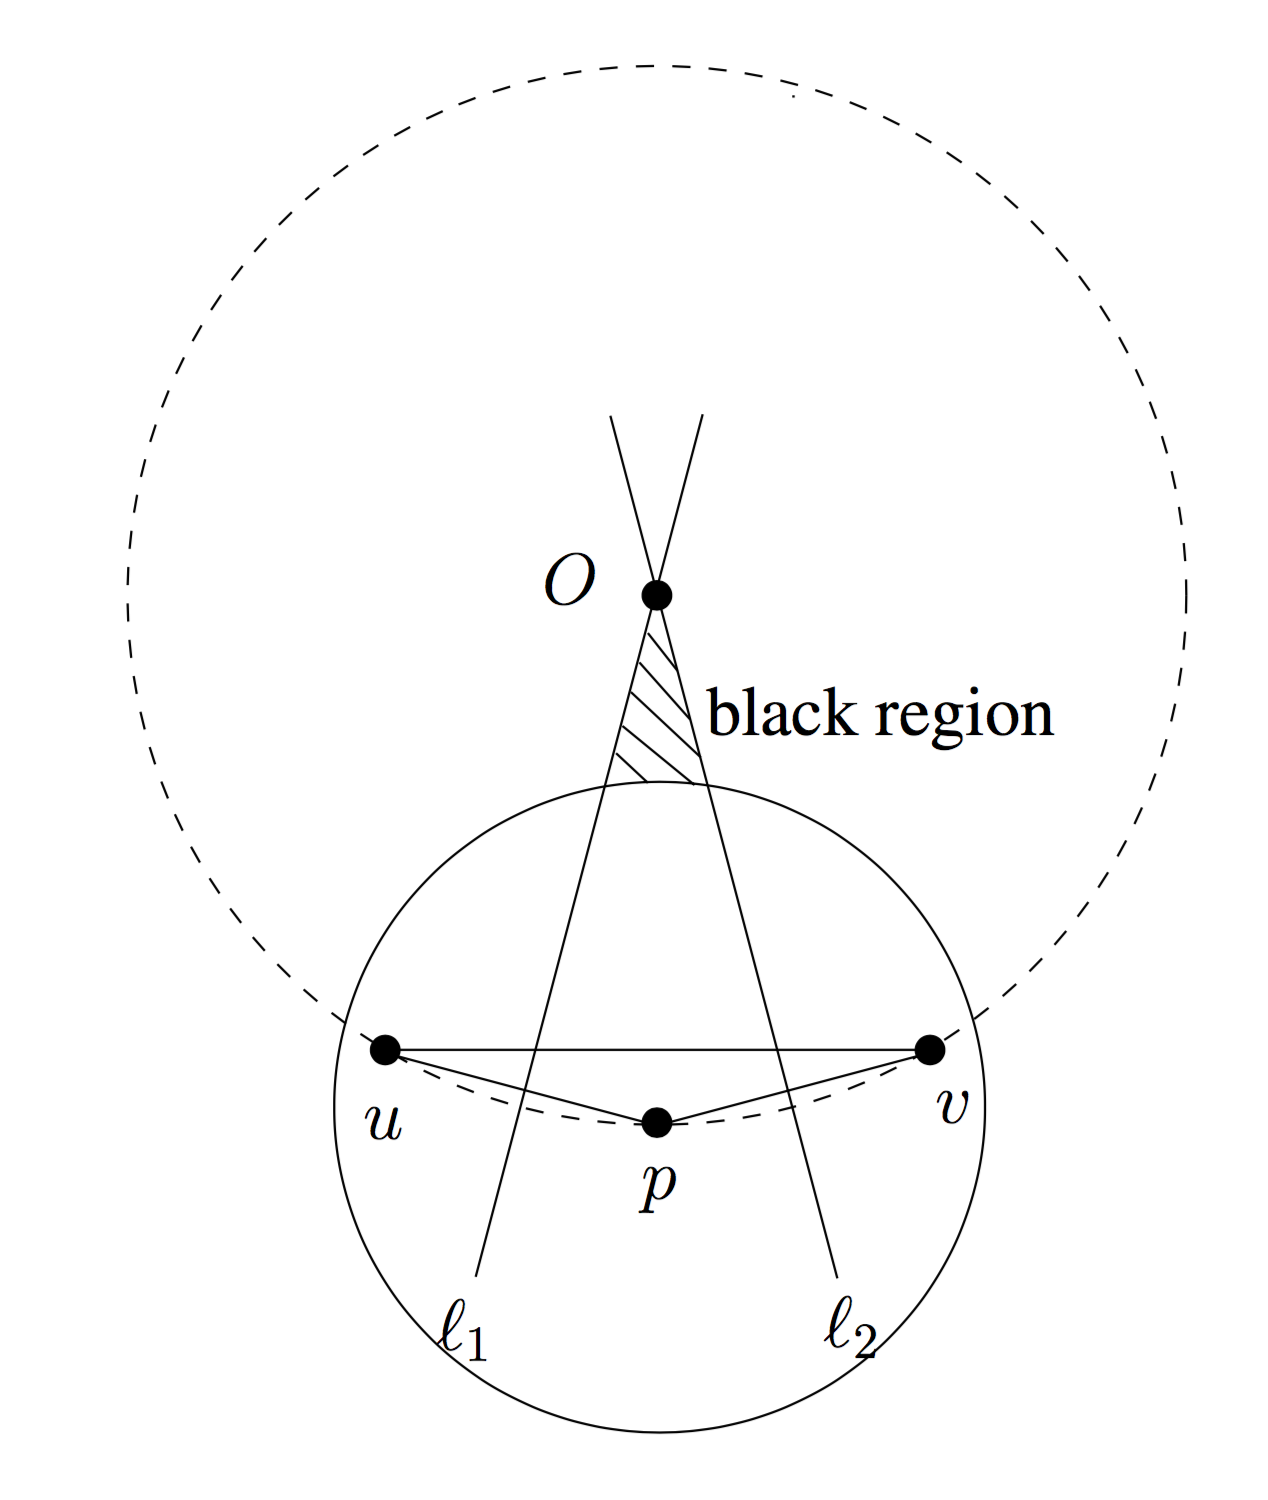
\includegraphics[width=0.4\textwidth]{Chapter3/Chapter3Figs/fig-stuck-node.png} % strongly stuck node
\caption{TENT rule: Node $p$ has no neighbors closer to the back regions as determined by the intersection of bisectors of adjacent links.}
\label{tent-rule}
\end{figure}

\subsection{The BOUNDHOLE algorithm}
After being detected as a \emph{stuck node}, the stuck node $p$ can initiate the distributed algorithm, \emph{BOUNDHOLE} that uses the right-hand rule to connect a node with its neighbors, to form a closed region. That closed region is a routing hole. The basic idea is shown in figure \ref{boundhole}. The algorithm starts from node $p$ and sweeps over the stuck direction by sending a packet to node $t_1$ in a counter-clockwise direction. Node $t_1$ then passes the packet to node $t_2$. The above process is repeated until the packet moves around the hole boundary and returns to $p$. Now that the boundary of a hole has been identified and stored locally. 

\begin{figure}[!htb]
\centering
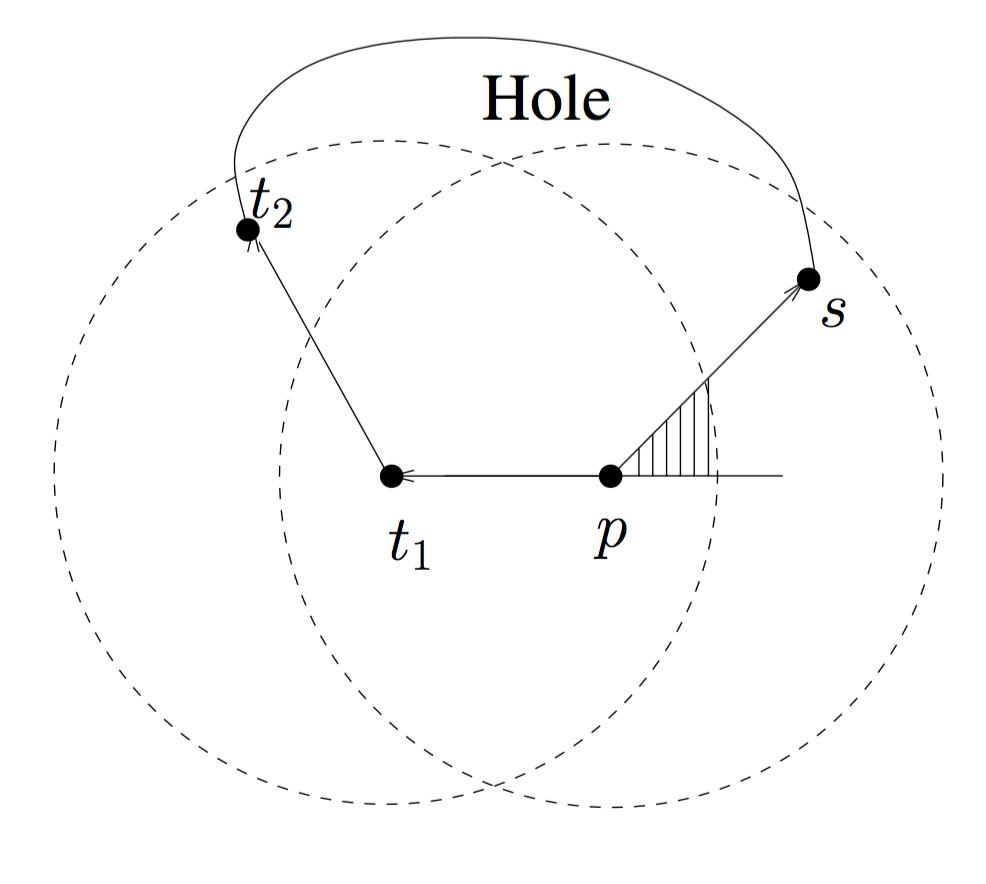
\includegraphics[width=0.4\textwidth]{Chapter3/Chapter3Figs/fig-boundhole.png} % strongly stuck node
\caption{BOUNDHOLE algorithm: Greedy sweeping at $t_1$}
\label{boundhole}
\end{figure}

A stuck node initiates a messenger packet in each direction this node is stuck in. Thus, there are a lot of packets the originated from all stuck nodes in the hole boundary. These packets are obviously redundant since we need only 1 packet to detect the hole boundary. To reduce networking overhead and possible packet collisions, especially when large holes exist in the network, the ID of the originator is recorded in each messenger packet and the messenger packet originated by the stuck node with the lowest ID is guaranteed to be overlaid at each hop. That is, all packets which have the originator ID greater than the lowest ID will be dropped.

Due to the distributed property of the \emph{TENT rule} and the \emph{BOUNDHOLE} algorithm, this protocol ensures the scalability even when the network topology is extended.

\section{Hole bypassing protocols}
As stated previously, all the proposed routing protocols using the \emph{BOUNDHOLE} algorithm in its hole boundary detection phase construct a forbidden area which covers the hole polygon. The purpose of constructing these forbidden areas is to simplify the hole polygon, thus it reduces the memory and network overhead for storing and broadcasting the hole information to the network. The forbidden area could be represented as a simpler shape such as circle \cite{ehds}, ellipse \cite{ellipse}, hexagon \cite{hexagon}, parallelogram \cite{elbar} or octagon \cite{issnip}. We call these simpler shapes are the approximate hole. These protocols are all separated to 2 main phases. The first one is the network initialization phase, and the second one is data forwarding phase. However, there are some fundamental differences among these protocols. 

In the network initialization phase, all mentioned protocols try to detect the hole boundary using the \emph{BOUNDHOLE} algorithm. After finishing detecting the hole boundary, the hole boundary message originator calculates the approximate holes. After that, some protocols (which are \cite{ellipse}, \cite{hexagon}, \cite{elbar}, \cite{issnip}) have an extra phase called broadcast hole information phase. The broadcast data could be the information of the approximate hole, and the broadcast area is controlled by a system parameter. In the contrary, some protocols (which are \cite{ehds}) forward the hole information to all boundary sensor nodes, and let each boundary sensor node calculate the approximate hole itself.

In the data forwarding phase, although each protocol uses a different shape of forbidden area, the routing path construction algorithm still shares some common ideas. They all use the concept of \emph{virtual anchor point}. These \emph{virtual anchor points} create a hole-bypassing routing path for the data packet, and its determination depends on each routing protocol. There are two common approaches to determine these \emph{virtual anchor points} which are: intersection points of tangent lines in case of \cite{ehds, ellipse} or vertices of approximate polygon in case of \cite{elbar, issnip, hexagon}. 

Due to the limitation of the thesis, we only give thorough studies on \cite{ehds,issnip,elbar} protocols.

%%% EHDS %%%
\subsection{The Efficient Hole Detour Scheme}
A representative for the group using the tangent line to construct the routing path is the Efficient Hole Detour Scheme (\emph{EHDS} protocol). In this proposal, the authors used a circumscribed circle to approximate the hole polygon.

In the network initialization phase, the protocol uses the \emph{BOUNDHOLE} algorithm to detect the hole boundary. Then the creator of the hole boundary detection message calculates the circumscribed circle of the hole polygon using the algorithm described in algorithm \ref{algo-circle}. This circumscribed circle information would be sent to all hole boundary sensor nodes. Figure \ref{fig-circle} represents the idea of this scheme. 

\begin{figure}[!htb]
\centering
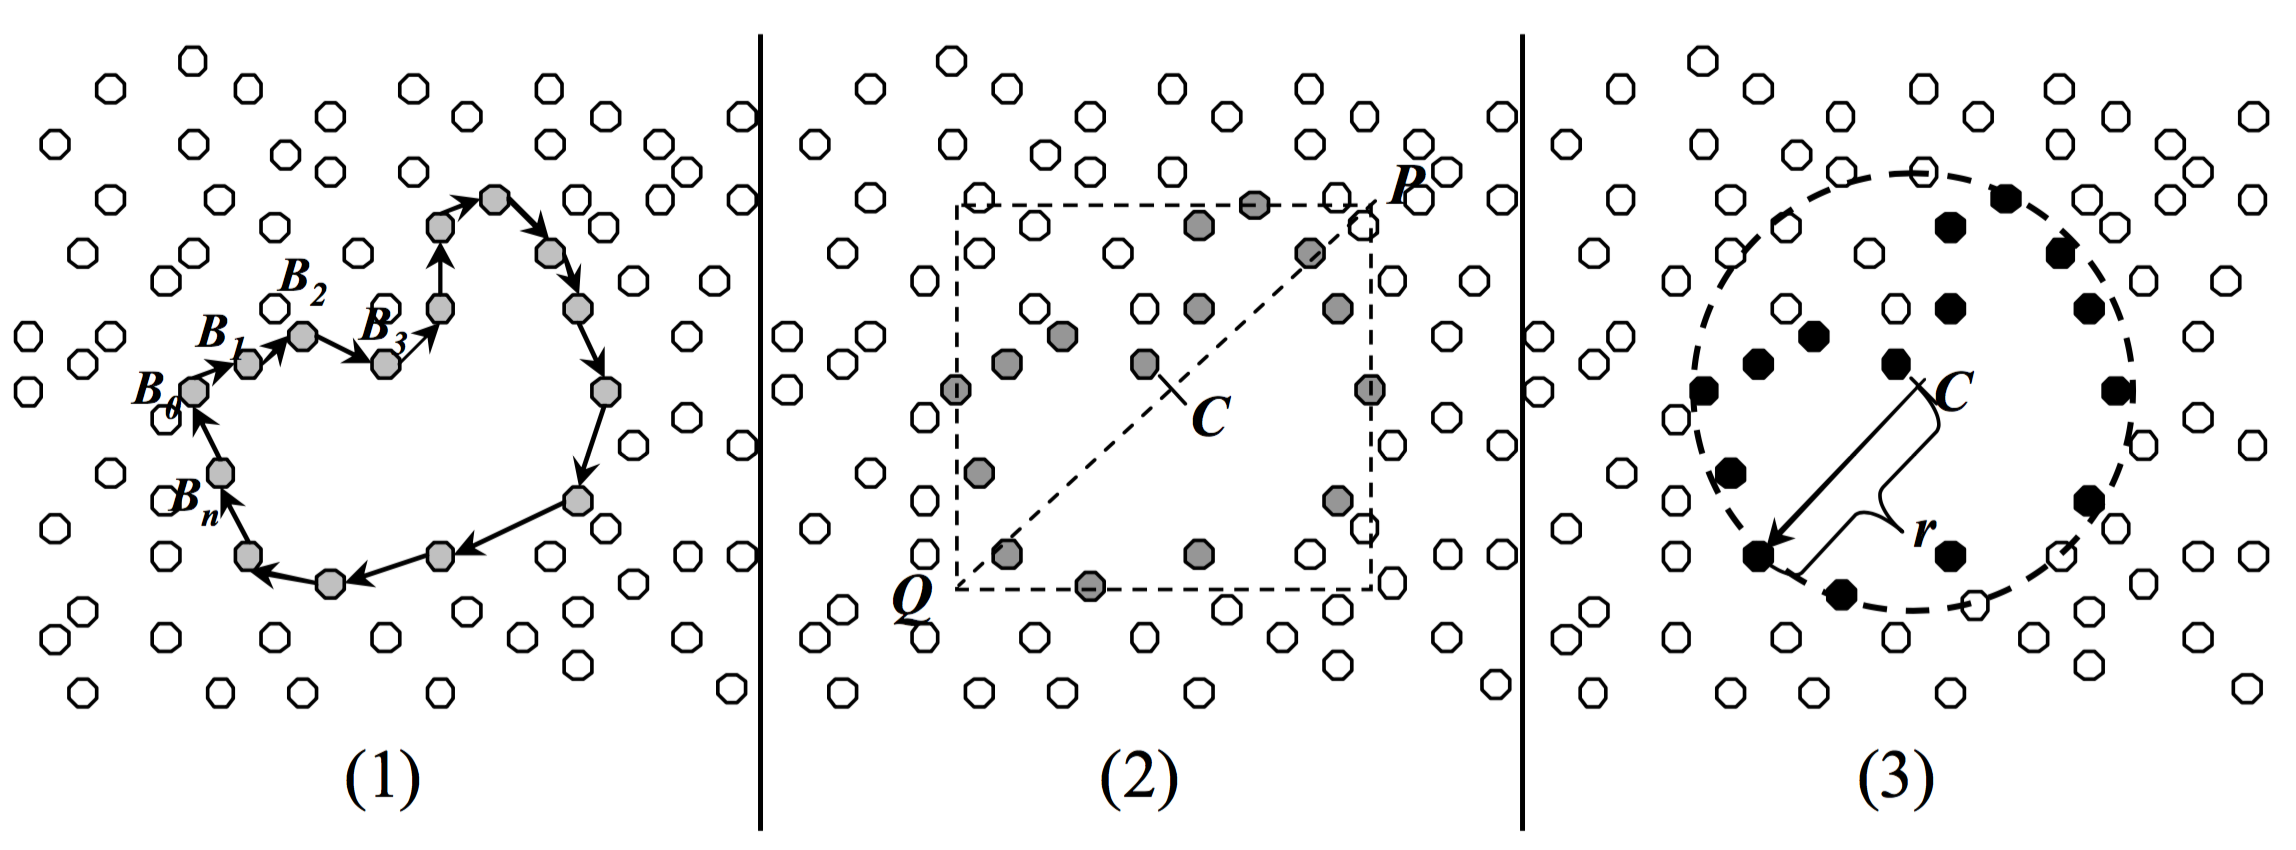
\includegraphics[width=0.6\textwidth]{Chapter3/Chapter3Figs/fig-circle.png}
\caption{The Efficient Hole Detour Scheme (cited from \cite{ehds}). Illustration for the hole approximation phase.}
\label{fig-circle}
\end{figure}

\begin{algorithm}[!htb]
\SetAlgoLined
\caption{Circumscribed circle constructing algorithm}
\label{algo-circle}
\Input{ $P=\left \{ P_1, ..., P_n \right \}$: the hole polygon}
\Output{$S(C, r)$: the circumscribed circle of $P$}

$X \leftarrow \{P_{i_x} \mid i = \overline{1,n}\}$\;
$Y \leftarrow \{P_{i_y} \mid i = \overline{1,n}\}$\;
$x_{min} \leftarrow min(X)$ \;
$x_{max} \leftarrow max(X)$ \;
$y_{min} \leftarrow min(Y)$ \;
$y_{max} \leftarrow max(Y)$ \;

$C \leftarrow (\frac{x_{min} + x_{max}}{2}, \frac{y_{min} + y_{max}}{2})$\;
$r \leftarrow \frac{\sqrt{(x_{min} - x_{max})^{2} + (y_{min} - y_{max})^{2}}}{2}$\;
\Return $S(C,r)$\;
\end{algorithm}

In the data forwarding phase, the packets are firstly forwarded by the greedy routing until it reaches a hole boundary sensor node. This node is called an intermediate node. This intermediate node would send the packet back to the source by greedy routing with extra information including the location of center point and the radius of the hole polygon's circumscribed circle. After finishing receiving back the packet, the source node resends the packet with new bypass routing path to avoid the circle. Figure \ref{fig-circle2} illustrates this routing protocol.

\begin{figure}[!htb]
\centering
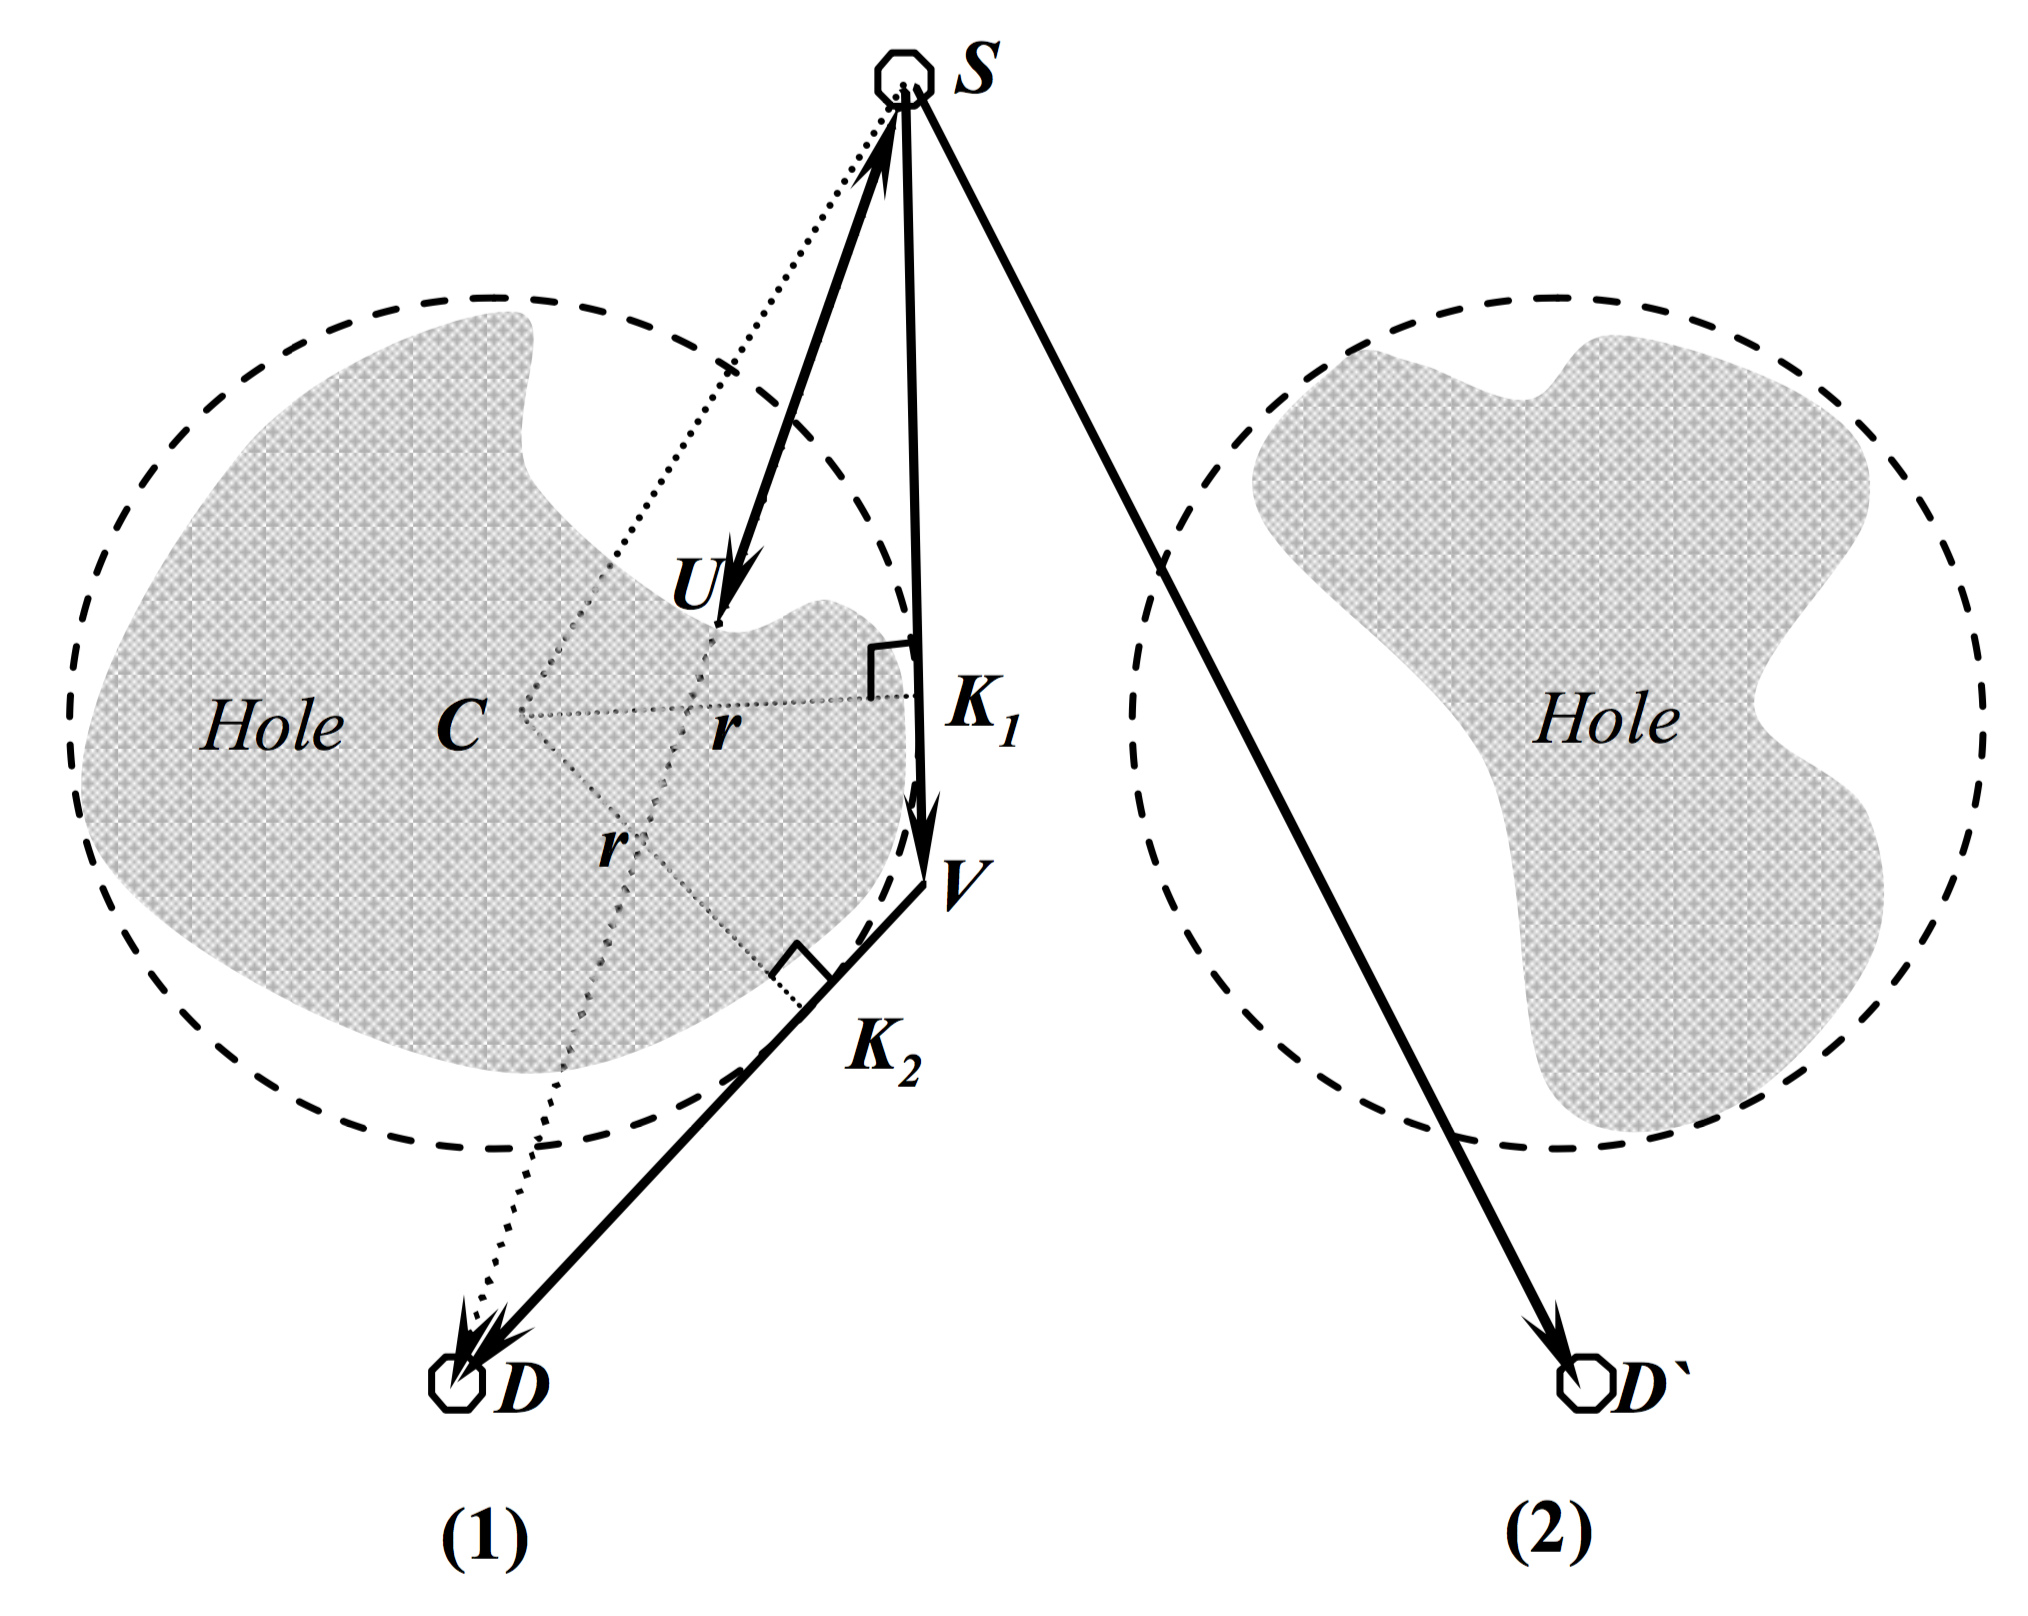
\includegraphics[width=0.4\textwidth]{Chapter3/Chapter3Figs/fig-circle2.png}
\caption{The Efficient Hole Detour Scheme (cited from \cite{ehds}). Illustration for the data forwarding phase. The forbidden area is the circumscribed circle of the hole polygon.}
\label{fig-circle2}
\end{figure} 

In this figure, \emph{S}, \emph{D} are the source node and the destination node, respectively. Firstly, \emph{S} greedily forwards the packet until it reaches a node \emph{U} which is a hole boundary sensor. \emph{U} then sends back to \emph{S} the forbidden area information. Finally, \emph{S} re-forwards the packet using new routing path, that is $\overrightarrow{SVD}$. The packet is forwarded along this path. \emph{V} is called the virtual anchor point in this case.

It is obvious that in the \emph{EHDS} protocol, the packet has to be forward twice: in the first time, it is forwarded by the greedy routing, in the second time, it is forwarded by the hole bypassing routing. Consequently, this increases the packet transmission time, as well as the energy consumption of nodes participating in the routing. 

One more problem of \emph{EHDS} protocol is that, this protocol leads to the routing path enlargement problem in case of near hole routing which is demonstrated in figure \ref{fig-circle-problem}.
\begin{figure}[!htb]
\centering
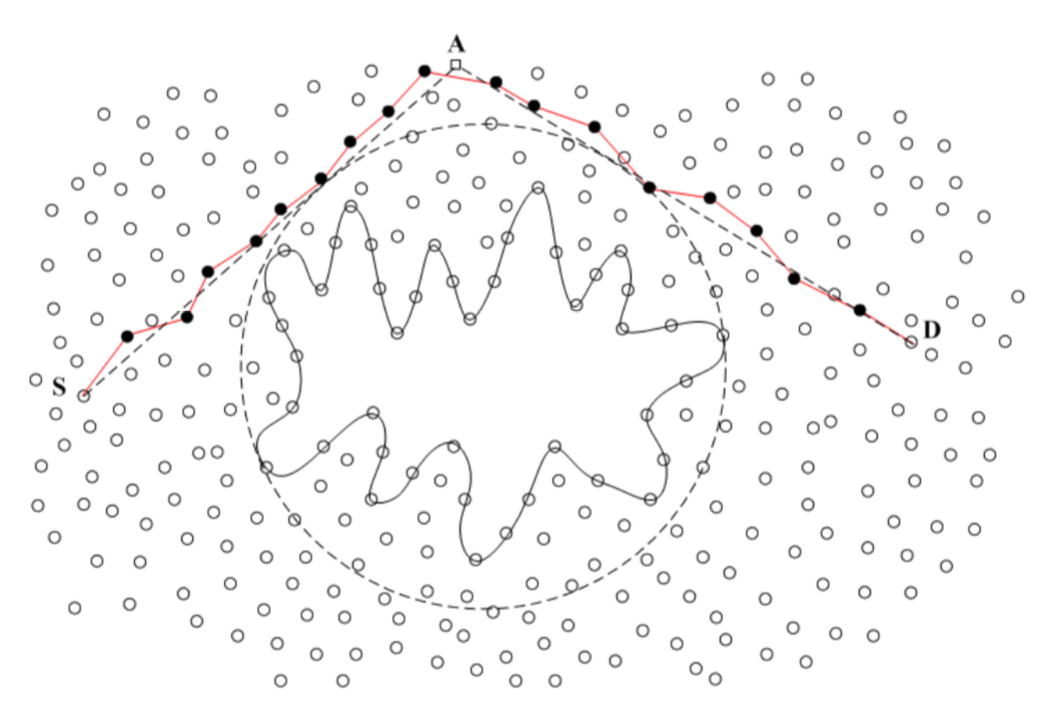
\includegraphics[width=0.4\textwidth]{Chapter3/Chapter3Figs/fig-circle-problem.png}
\caption{The routing path is enlarged in case of near hole routing.}
\label{fig-circle-problem}
\end{figure}

In this figure, the source node \emph{S} is close to the forbidden area. Since this protocol uses the tangent line as the routing path, the closer to the forbidden area the source node and the destination node are, the more longer the routing path is.

More importantly, the author ignored the case where the source node or the destination node or both of them are inside the forbidden area. In such a case, there is no hole bypassing routing paths.

%%% ELBAR %%%
\subsection{The Energy Efficient and Load Balanced Distributed Routing Scheme}
The Energy Efficient and Load Balanced Distributed Routing Scheme (ELBAR protocol) is the one that simultaneously considers both energy efficiency and load balancing requirements. 
In this protocol, the authors proposed a novel algorithm to approximate the hole polygon. Instead of using a geometric shape, the authors use a square grid to approximate the hole \cite{gridoffline}. Using a square grid ensures the convex/concave properties of the original hole polygon, and the error between the approximate hole and original hole is controlled by a system parameter which is the length of edges of grid's square units. The approximate hole is a polygon whose edges are the edges of the grid and vertices are the vertices of the grid. Its properties are:
\begin{itemize}
\item Covering: the approximate hole covers completely the hole polygon.
\item Controllable approximate error: the upper bound of the total vertices of the approximate hole is controlled by a system parameter $n$. The larger the value of $n$ is, the less the approximate error is.
\end{itemize}

\begin{figure}[!htb]
\centering
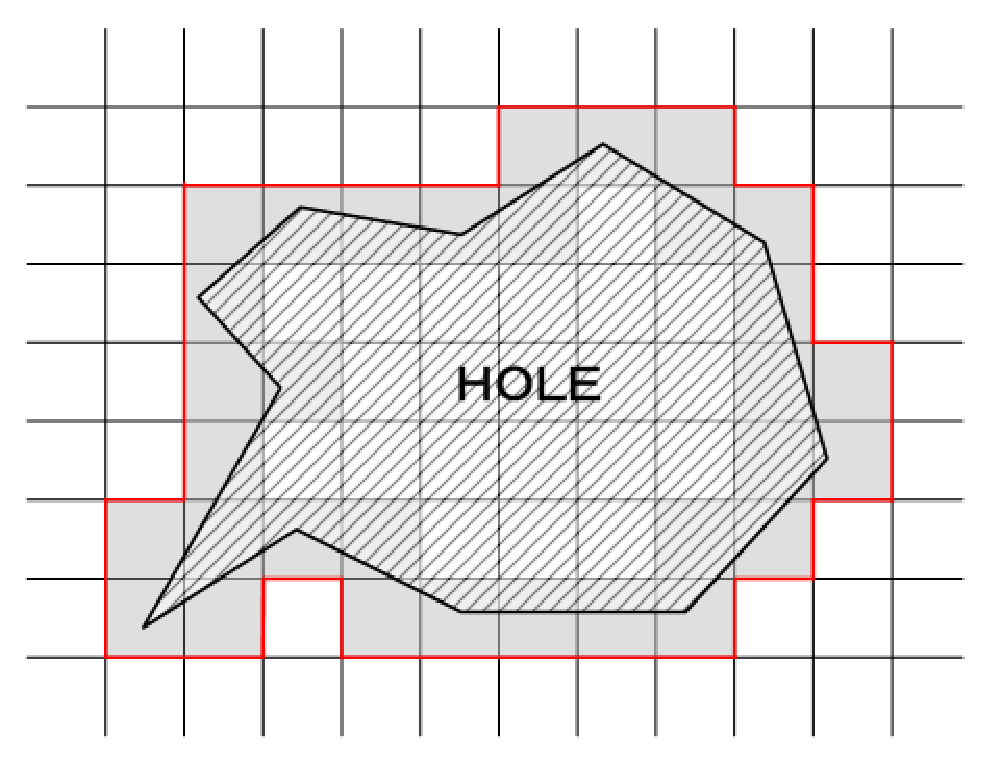
\includegraphics[width=0.5\textwidth]{Chapter3/Chapter3Figs/fig-elbar-grid.eps}
\caption{An example of approximate polygon.}
\label{fig-elbar-grid}
\small{Grey area represents the hole. Bold black line represents the boundary of the approximate polygon.}
\end{figure}
Figure \ref{fig-elbar-grid} illustrates the approximate hole using a square grid.

This scheme propose additional modifications to the packet forwarding function and routing functions. With respect to specific routing hole H all the nodes are divided into three regions based on two predefined threshold values $\alpha_{min}$ and $\alpha_{max}$ as shown in figure \ref{fig-elbar-regions}. A particular node is in:
\begin{itemize}
\item region 1 if the hole view angle of the node is either greater than or equal to $\alpha_{max}$,
\item region 2 (which is referred to as an escape region in what follows) if the hole view angle of the node is in interval $(\alpha_{min}, \alpha_{max})$,
\item region 3 if the hole view angle of the node is either less than or equal to $\alpha_{min}$.
\end{itemize}

\begin{figure}[!htb]
\centering
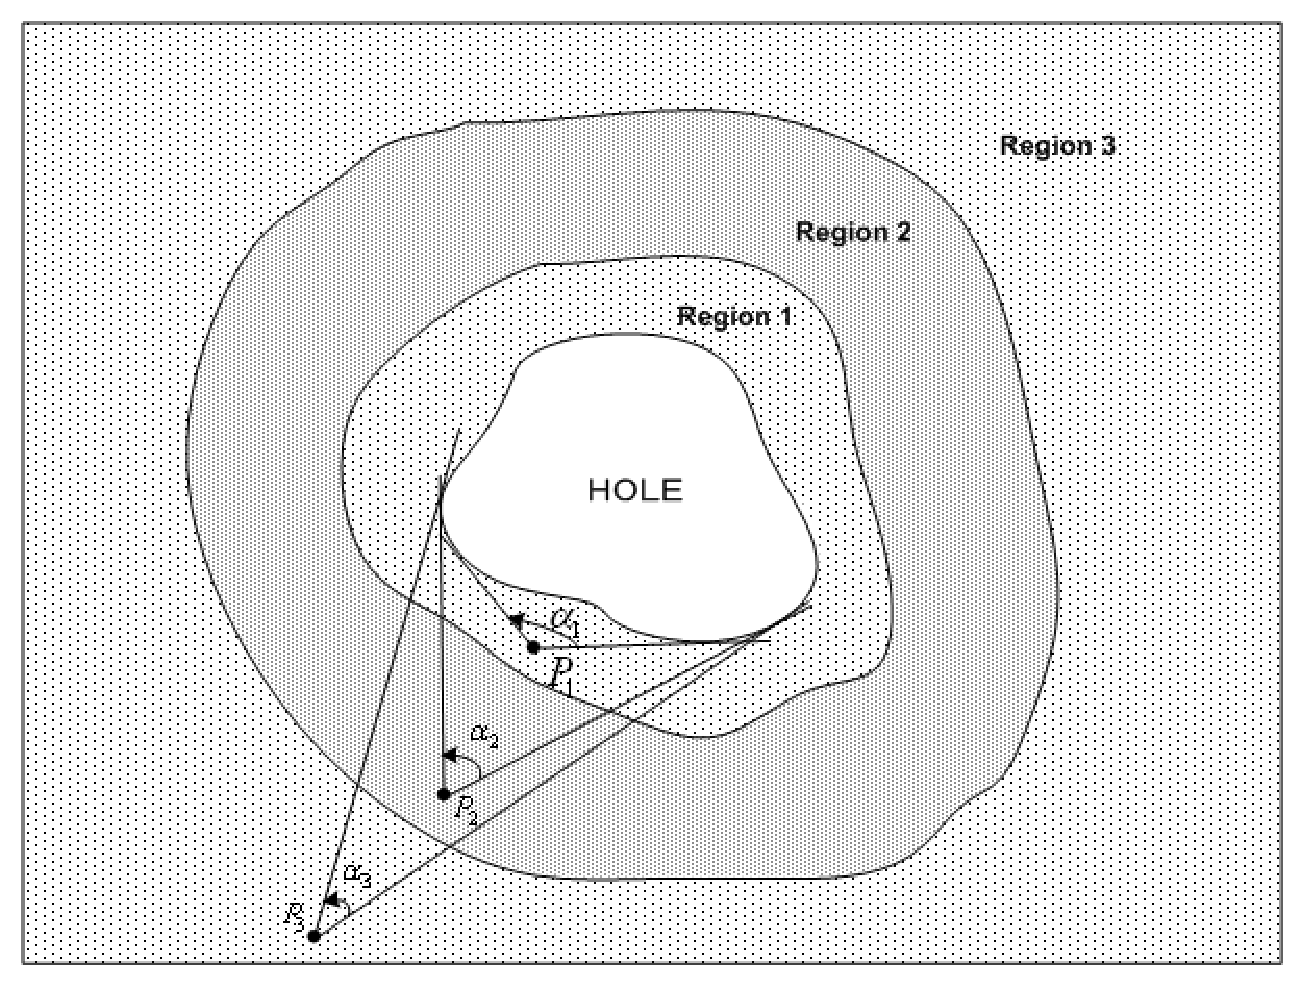
\includegraphics[width=0.5\textwidth]{Chapter3/Chapter3Figs/fig-elbar-regions.eps}
\caption{Regions with respect to a specific routing hole.}
\label{fig-elbar-regions}
\end{figure}

A parallelogram is used as the forbidden area, and these parallelograms are different from each sensor node. The construction of the parallelogram is illustrated in figure \ref{fig-elbar-parallelogram}.

\begin{figure}[!htb]
\centering
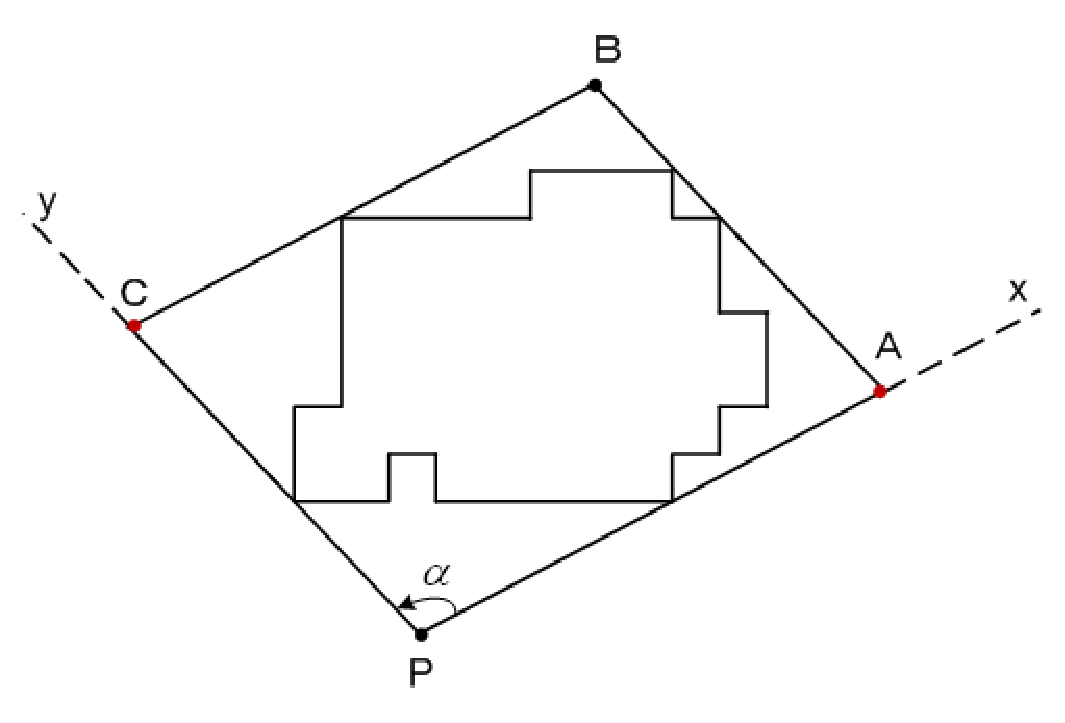
\includegraphics[width=0.5\textwidth]{Chapter3/Chapter3Figs/fig-elbar-parallelogram.eps}
\caption{The parallelogram of the sensor node $P$}
\label{fig-elbar-parallelogram}
\end{figure}

The routing protocol is described as follows. Two fields are proposed to be carried by a packet: the first field is the \emph{forwarding mode} that can take either \emph{default} or \emph{escape} value, while the second field \emph{anchor location} is to store the anchor point in the \emph{escape} mode. Let $D$ be the destination of packet $p$. The forwarding mode $p_m$ is initialized to \emph{default} and anchor location $p_a$ takes $D$ when packets are first generated. When node $P$ is in region 3, it simply keeps the \emph{default} mode. When $P$ is in the \emph{escape} region and
\begin{itemize}
\item if $D$ lies either outside the hole view angle of $P$ or inside the hole covering parallelogram at $P$, then the packet is forwarded by the rule of the GPSR protocol \cite{gpsr}.
\item otherwise, a hole escape probability function is executed to adjust the routing mode for the packet. In the escape mode, the route is ``bended'' around $P$’s hole view parallelogram.
\end{itemize}

\begin{figure}[!htb]
\centering
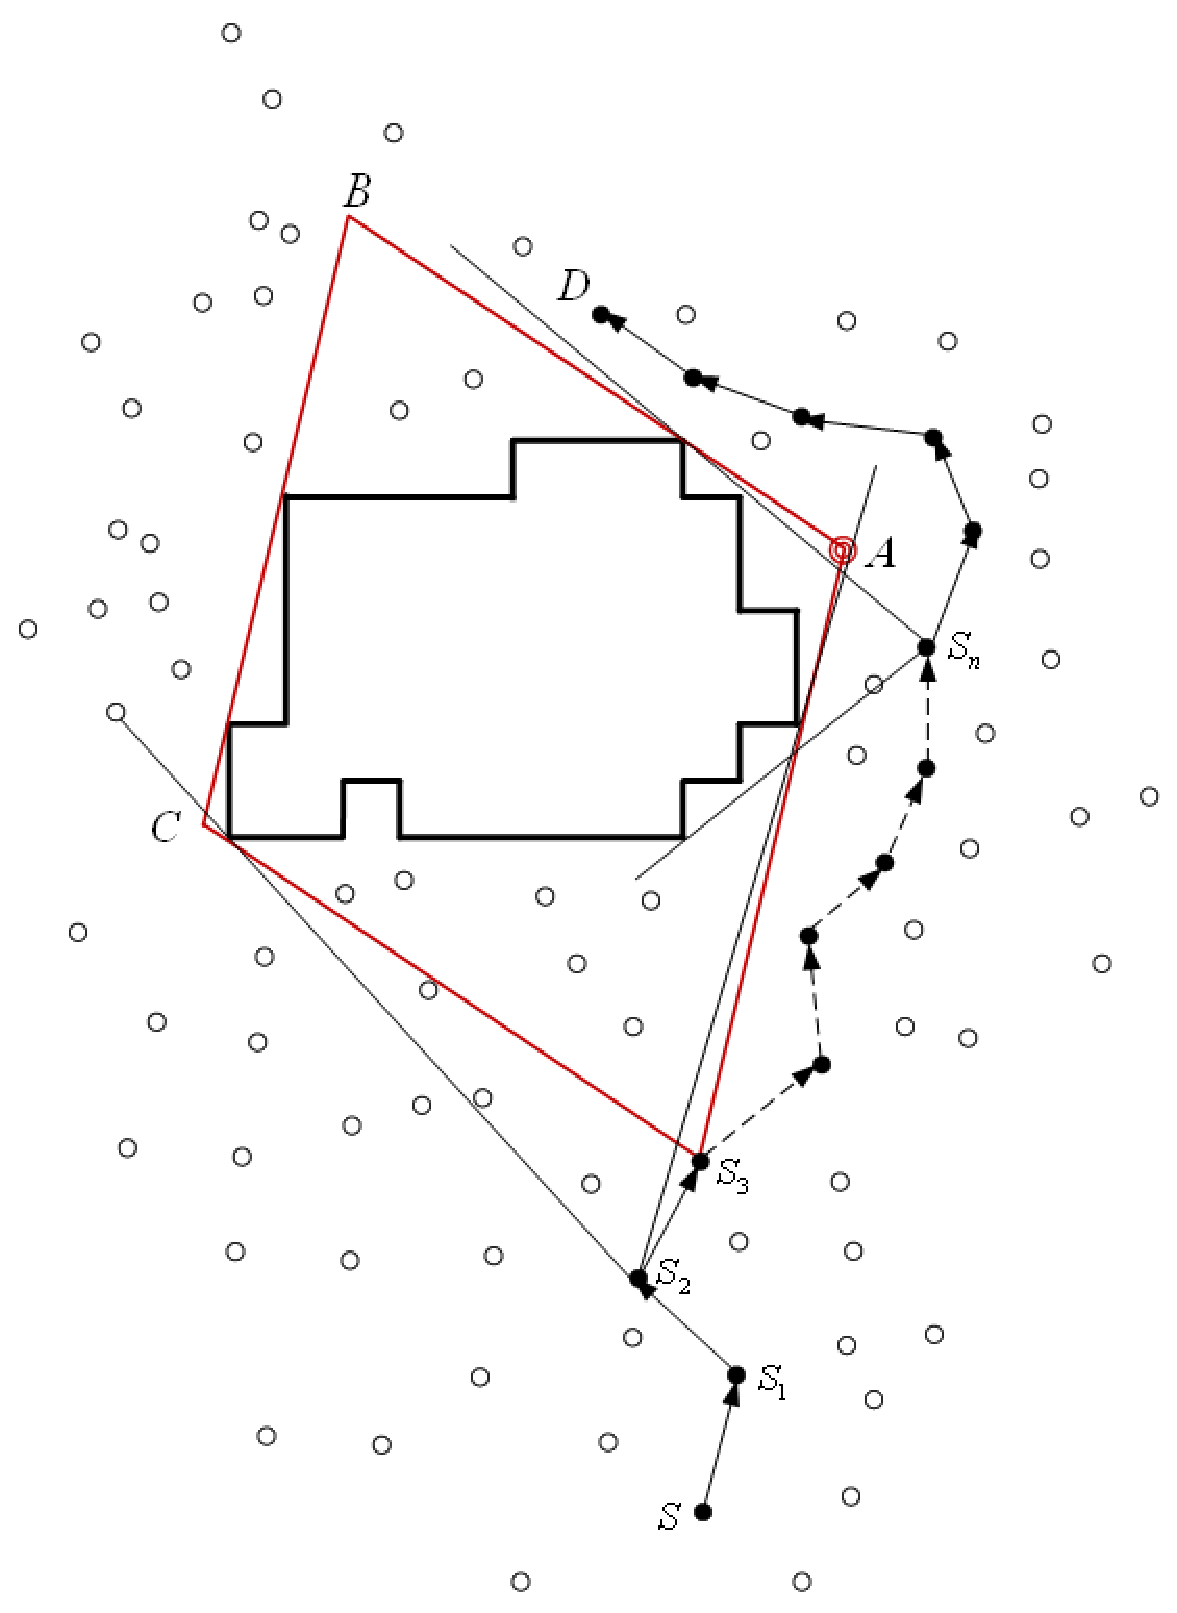
\includegraphics[width=0.5\textwidth]{Chapter3/Chapter3Figs/fig-elbar-routing.eps}
\caption{ELBAR packet forwarding example.}
\label{fig-elbar-routing}
\end{figure}

Figure \ref{fig-elbar-routing} illustrates how a data packet would be routed from source node $S$ in region 3 to destination node $D$. When in region 3 (far from the hole then has no information about it) the packet is forwarded in the \emph{default} mode until it reaches a node in region 2, namely node $S_2$ in the figure. Note that reaching region 2 does not mean automatically switching to \emph{escape} mode but to mean having a chance to switch to this mode. In this example, the adjust routing mode method at $S_2$ returns in \emph{default} mode, thus the packet is forwarded to the neighbor of $S_2$ which is nearest to destination $D$. However, at the next hop, i.e $S_3$, the adjust routing mode method returns in \emph{escape} mode thus $S_3$ updates necessary fields and sends the data packet towards the virtual anchor $A$. Before arriving to the node which is nearest to $A$, the packet however reaches intermediate node $S_n$ that can “see” $D$ (without the view blocking of the hole). Now $S_n$ forwards the packet in the default mode to destination $D$.

In the \emph{ELBAR} protocol, we can think region 1 as the near hole region. For the source node belonging to this region, the \emph{GPSR} routing protocol is used.

%%% ISSNIP %%%
\subsection{The Load Balanced Routing with Constant Stretch Scheme}
The Load Balanced Routing with Constant Stretch Scheme (the \emph{OCTAGON} protocol) takes a further step to target and solve two problems of hole diffusion and path enlargement. Its theoretical analysis proves the constant stretch property and its evaluation results show that this scheme strongly outperforms the existing schemes in several performance factors, including route stretch, efficient use of energy and load balancing.

This protocol also consists of 2 main phases: the initial network setup phase and the data forwarding phase. The initial network setup is designed to produce the core polygon, a compact approximation of the hole, which has 8 vertices and covers the hole boundary. The initial network setup process consists of three sub-phases. First, the nodes on the hole boundary are identified using the \emph{BOUNDHOLE} algorithm \cite{boundhole}. Then, the core polygon is constructed. In the final phase, the core polygon information is disseminated to the nodes surrounding the hole. The dissemination area is not all of the network but only a restricted area in order to save the energy consumption. Once the initial network setup is finished, the nodes nearby the hole know about the location of the core polygon while the nodes far from the hole do not.

If the packet is initialized at a source node out of a dissemination area of a hole(not knowing about the hole and the core polygon), it is simply greedily forwarded towards the destination node until reaching an intermediate node inside this area. Once in this area the source node (or intermediate node) can construct a packet-specific polygon, seen as a forbidding area for this packet, which is the image of the core polygon through a homothetic transformation with the scale factor based on the source-destination distance. The packet is then greedily forwarded to the virtual anchor points which are the vertices of this packet-specific polygon. 

The core polygon satisfies the following conditions:
\begin{itemize}
\item It completely covers (the boundary of) the hole.
\item It has at most 8 vertices and each edge of its contains at least one vertex of the hole.
\item All angles at the vertices that are not the vertices of the hole, equal to $\frac{3\pi}{4}$.
\end{itemize}

After the core polygon information broadcast phase, the network is divided into 2 regions: region 1 contains nodes that receive the hole core polygon broadcast message, and region 2 contains the other nodes as shown in figure \ref{fig-issnip-routing}.

The main idea of the data forwarding phase is to find the shortest route that has to go around a larger polygon $A$ that is the image of the core polygon through a homothetic transformation using a center $I$ chosen randomly inside the core polygon and the scale factor $\xi > 1$ computed based on the distance between the source and the destination. This polygon $A$ is being used as a dynamic forbidding area which is different per each packet and source node because of the randomization of center $I$. As a result, the routing path also changes dynamically for each packet and thus balance the energy consumption of the network. While, the scale factor $\xi$ is designed so that the stretch of the routing path is bounded by a constant. Figure \ref{fig-issnip-routing} shows examples of the routing scheme in both cases when the source node belongs to the region 1 and to the region 2.

\begin{figure}[!htb]
\centering
\begin{subfigure}{0.5\textwidth}
  \centering
  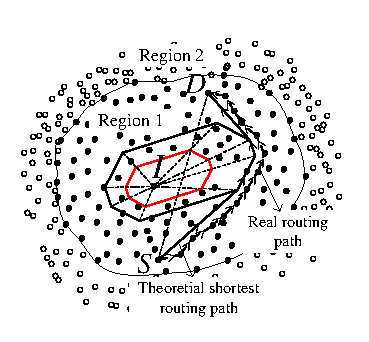
\includegraphics[width=0.8\textwidth]{Chapter3/Chapter3Figs/fig-issnip-routing1.eps}
  \caption{Source node belongs to region 1}
  \label{fig-issnip-routing1}
\end{subfigure}%
\begin{subfigure}{0.5\textwidth}
  \centering
  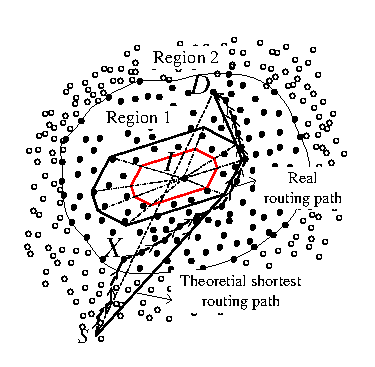
\includegraphics[width=0.8\textwidth]{Chapter3/Chapter3Figs/fig-issnip-routing2.eps}
  \caption{Source node belongs to region 2}
  \label{fig-issnip-routing2}
\end{subfigure}
\caption{Examples of the \emph{OCTAGON} routing scheme}
\label{fig-issnip-routing}
\end{figure}

Since our near hole routing protocol adopted some advantages from this protocol, we give here more details about this protocol's theoretical analysis. Firstly, the authors proved that the upper bound of the stretch does not exceed $\frac{1}{sin(3\pi /8)} + \delta$ for every source and destination pair $(S, D)$ staying outside the core polygon. More notably, the authors explained the reason why they choose a octagon to approximate the forbidden area. The reason is if $P$ is a \emph{n-gon} with equal angles such that $P$ covers the hole and each edge of $P$ contains at least one vertex of the hole, then the E-stretch of $P$ to the hole is bounded by $\frac{1}{sin(\frac{(n-2)\pi}{n})}$, a decrease function which converges to 1. The value of this function decreases strongly when $n$ increases from 3 to 8 and does not decrease much after that.
\chapter{Near hole routing protocol}\label{chapter4}
In this chapter, we describe our near hole routing protocol in details. 
\section{Proposed Scheme}
\subsection{Assumptions and definitions}
To ease the comprehension, we present a short overview of terms and definitions related to routing holes. Following the approach in \cite{ehds,elbar,issnip}, we consider the same assumptions as follows.
\begin{itemize}
\item Each node knows the position of itself and its 1-hop neighbors by using GPS or other positioning services.
\item The location of a destination is known by a source.
\item All the sensor nodes have the same radio hardware. Let $R_c$ denote the transmission range of a node.
\item The energy consumption of the computation performed for one packet at a node is negligible compared to the energy consumption of the transmission of one packet.
\end{itemize}
We start with the definitions of the notations and terms being used throughout this paper. Below, let $P$ denote a polygon which is determined by a set of vertices $P_1, P_2, ..., P_n$.

\begin{mydef}[Convex hull of polygon]
The convex hull of polygon $P$ is the smallest polygon whose vertices are vertices of $P$ and completely covers $P$.
\end{mydef}
The convex hull of polygon $P$ is denoted as $C_P$.

\begin{mydef}[View-limit vertex]\label{def-view-limit-vertex}
$P_i$ is called a view-limit vertex from a point $N$ outside $P$ to $P$ if and only if the line through $N$ and $P_i$ does not intersect $P$ (see Figure \ref{fig-def-viewlimit}).
\end{mydef}
Clearly, there are only two such view-limit vertices from a given node $N$.

\begin{figure}[!htb]
\centering
\begin{subfigure}{0.5\textwidth}
  \centering
  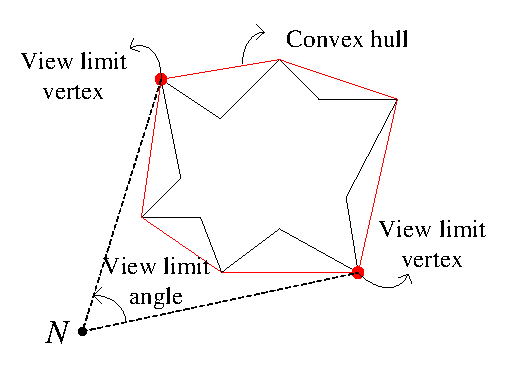
\includegraphics[width=0.6\textwidth]{Chapter4/Chapter4Figs/fig-view-limit-vertex.eps}
  \caption{View-limit vertices of $N$}
  \label{fig-def-viewlimit}
\end{subfigure}%
\begin{subfigure}{0.5\textwidth}
  \centering
  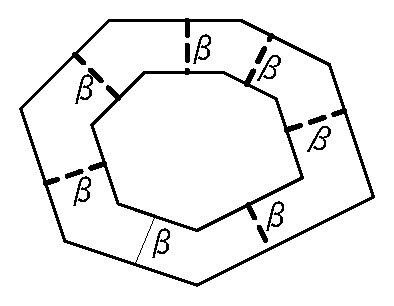
\includegraphics[width=0.6\textwidth]{Chapter4/Chapter4Figs/fig-covering-polygon.eps}
  \caption{$\beta$-covering polygon}
  \label{fig-def-betacovering}
\end{subfigure}
\caption{Illustrations of definition \ref{def-view-limit-vertex}, \ref{def-beta-covering}}
\label{fig-beta-covering}
\end{figure}

\begin{mydef}[$\beta$-covering]\label{def-beta-covering}
Assume that $P$ is a polygon and $\beta$ is a positive number. Then, $\beta$-covering polygon of $P$ is a polygon covering $P$ and having each edge parallels to an edge of $P$ while the distances between each parallel pair is the same $\beta$ (see Figure \ref{fig-def-betacovering}).
\end{mydef}

\begin{mydef}[Point-to-Polygon Distance]
Assume that $P$ is a convex polygon, $N$ is a point staying outside of $P$ . $d > 0$ is defined as the distance from $N$ to $P$ if and only if $N$ stays on the boundary of $d$-covering polygon of $P$.
\end{mydef}
The distance from point $N$ to polygon $P$ is denoted as $d(P, N)$.

\begin{mydef}[Inner polygon]
An inner polygon of polygon $P$ is a set of sequentially ordered nodes denoted by $IP_{P_{jk}} = \{ P_j, P_{j+1}, ..., P_k\}$, where $IP_{P_{jk}} \in P$ such that $P_j$ and $P_k$ are the extreme points of convex hull $C_P$. In particular, $P_jP_k$ is called the \textbf{gateway} of $IP_{P_{jk}}$.
\end{mydef}
Figure \ref{fig-def-inner} shows an example with four inner polygons and their gateways. There is a polygon $P$ (black edges). Polygon $P$ has four inner polygons which are $IP_1$, $IP_2$, $IP_3$, $IP_4$. The gateway of $IP_1$, $IP_2$, $IP_3$, $IP_4$ are $IP_{1_1}IP_{1_2}$, $IP_{2_1}IP_{2_2}$, $IP_{3_1}IP_{3_2}$, $IP_{4_1}IP_{4_2}$ (red edges), respectively.

\begin{figure}[!htb]
\centering
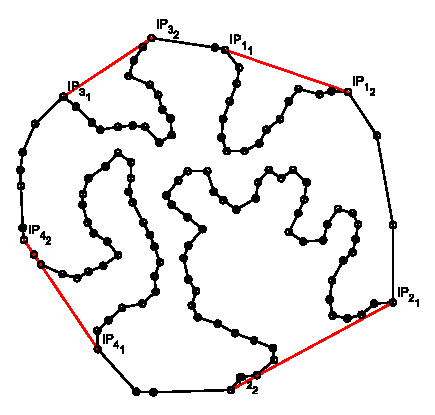
\includegraphics[width=0.3\textwidth]{Chapter4/Chapter4Figs/fig-innerpolygon.eps}
\caption{An example of inner polygons.}
\label{fig-def-inner}
\end{figure}

\subsection{Overview}
Our proposed scheme consists of two parts, namely the \emph{initial network setup} and the \emph{data forwarding}. The \emph{initial network setup} is designed to construct a graph for each inner polygon of the hole polygon. It consists of three phases: \emph{Hole Boundary Detection}, \emph{Hole Information Dissemination} and \emph{Internal Graph Construction}. Firstly, in the \emph{Hole Boundary Detection} phase, the hole boundary is identified using the \emph{BOUNDHOLE} algorithm \cite{boundhole}. During this phase, a leader node who is responsible for initiating the next phase: \emph{Hole Information Dissemination} is selected based on node IDs. This leader node also determines the convex hull of the hole polygon. Then, in the \emph{Hole Information Dissemination}, the hole polygon information is disseminated to the nodes surrounding the hole. The dissemination area is controlled by a system parameter $\delta$. The dissemination area is called the \textbf{near hole region}. Finally, in the \emph{Internal Graph Construction}, all nodes staying inside any inner polygons build an internal graph of its inner polygon. The internal graph is built based on the Voronoi diagram \cite{voronoi} of the inner polygon. It represents the internal structure of a inner polygon and is used for routing a packet optimally inside the convex hull of a hole.

Our data forwarding algorithm provides two routing mode, namely, \emph{near hole} mode and \emph{default} mode. The near hole routing consists of three cases:
\begin{itemize}
\item Both source node and destination node belong to the \emph{near hole region}.
\item Only source node belongs to the \emph{near hole region}.
\item Only destination node belongs to the \emph{near hole region}.
\end{itemize}

In the first case, the source node $s$ uses the \emph{near hole} mode to guide a packet out of the convex hull. If $s$ stays inside any inner polygons, it first finds an intermediate node in the \emph{gateway} and deliveries the packet to it. We call this intermediate node the source's \textbf{virtual anchor point} (VA-point). The detail algorithm to compute the VA-point is described in the next subsections. Otherwise, $s$ is the source's VA-point itself. In the source's VA-point, a \emph{dynamic forbidden area}, seen as a packet-specific forbidden area, is constructed. It is the image of the octagon covering the hole polygon through a homothetic transformation with the scale factor based on the distance from the source's VA-point to the convex hull. It also checks that if the destination node $d$ is inside any inner polygons. If the answer is ``yes'', it constructs the internal graph of the inner polygon containing $d$ and determines the destination's VA-point. The packet is then greedily forwarded to the VA-points which are the vertices of this packet-specific polygon. When the packet reaches the last VA-points, it is keeps greedily forwarding the packet to the destination's VA-point. Finally, the destination's VA-point forwards the packet to the destination based on the constructed internal graph. 
Figure \ref{fig-nhr-routing} shows an example of this case. In this figure, $I_s$ is the VA-point of the source node $s$, $I_1, I_2, I_3$ is the VA-points which are the vertices of scale octagon, and $I_d$ is the VA-point of the destination node $d$. The routing path is $\overrightarrow{sI_sI_1I_2I_3I_dd}$.

\begin{figure}[!htb]
\centering
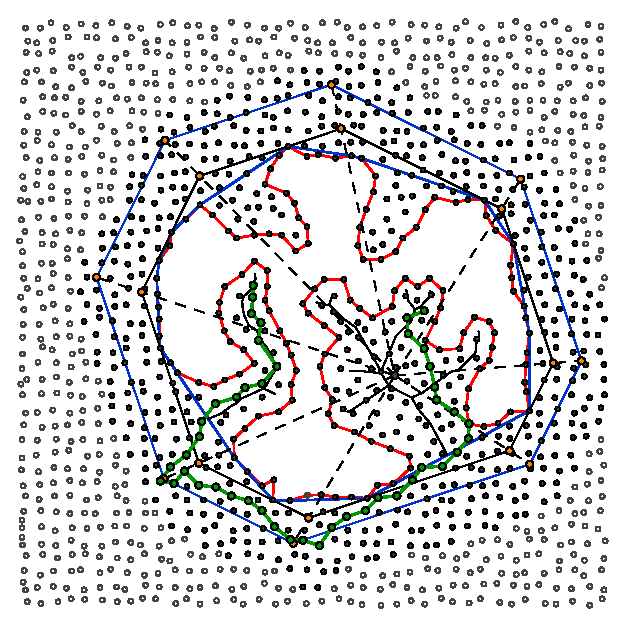
\includegraphics[width=0.4\textwidth]{Chapter4/Chapter4Figs/fig-path-example.eps}
\caption{An example of proposed routing path.}
\label{fig-nhr-routing}
\end{figure}

In the second case, the packet is forward along the routing path constructed same as the first case, until it reaches an intermediate node that does not belong to the \emph{near hole region}. Then the packet is greedily forwarded to destination node. In the third case, first, the packet is forward greedily to the destination, until it reaches an intermediate node belonging to the \emph{near hole region}. The routing path from this intermediate node to destination node is constructed same as the first case. In two later cases, the near hole routing protocol is used to find the path from the source to the intermediate node or from the intermediate node to the destination.

The detailed scheme is described in the following subsections.

\subsection{Hole Boundary Detection}
The \emph{TENT rule} is executed to identify the node on the hole boundary. Then, the \emph{Hole Boundary Detection} (\emph{HBD}) packet is formed and forwarded around the hole boundary using the \emph{BOUNDHOLE} algorithm. Assume $H_0$ is the leader node of the hole. After the \emph{HBD} packet came back to $H_0$, it has the information of all hole boundary sensor node $H_0, H_1, H_2, ..., H_n$. $H_0$ then uses the \emph{Graham scan} algorithm to determine the convex hull of the hole polygon. The information of each hole boundary sensor node is stored as format described in table \ref{table-node-info}.

\begin{table}[!htb]
\centering
\caption{Storage scheme of a hole boundary sensor node.}
\label{table-node-info}
\begin{tabular}{|l|l|}
\hline
x              & x-coordinate of node                                          \\ \hline
y              & y-coordinate of the node                                      \\ \hline
isExtremePoint & true if it is a vertex of the convex hull and false otherwise \\ \hline
\end{tabular}
\end{table}

\subsection{Hole Information Dissemination}
After the convex hull construction, node $H_0$ then creates a hole polygon information (\emph{HPI}) message that stores the information of the polygon vertices (which is the format described in table \ref{table-node-info}), and disseminates this \emph{HPI} message to its neighbors. In addition, to reduce the overhead of transmission information, before disseminating, $H_0$ will try to eliminate the vertices of any inner polygons whose vertices number is less than the system parameter $\eta$ (our experiments show that with an appropriately chosen value of $\eta$ (e.g., $\eta = 10$), it reduces the message overhead and still ensures the routing mechanism). This eliminating algorithm is described in algorithm \ref{alg-reduce-polygon}. 

\begin{algorithm}[!htb]
\SetAlgoLined
\caption{Hole polygon's vertices eliminating algorithm}
\label{alg-reduce-polygon}
\Input{$P = \{P_1, P_2, ..., P_n\}$: the linked list of the hole polygon vertices in counterclockwise order.\newline
$\eta$: pre-defined system parameter.}
\Output{$P$: simplified hole polygon.}
\For{$i = 1$ \KwTo $n$} {
	\uIf{$P[i].isExtremePoint = false$} {
		Remove $P[i]$ from $P$\;
		Append $P[i]$ to the end of $P$\;
	}
	\lElse {
		\KwBreak
	}
}
\For{$i = 1$ \KwTo $n$} {
	\If{$P[i].isExtremePoint = true$} {
		$j \leftarrow 0$\;
		$m \leftarrow i$\;
		\While{$P[i+1].isExtremePoint = false$} {
			$j \leftarrow j + 1$\;
			$i \leftarrow i + 1$\;
		}
		$i \leftarrow i - 1$\;
		\lIf{$j \leq \eta$} {
			Remove $\{P_{m+1}, P_{m+2}, ..., P_{i}\}$ from $P$
		}
	}
}
\Return $P$\;
\end{algorithm}

When an intermediate node $N$ receives this \emph{HPI} message, it does following tasks:
\begin{itemize}
\item Stores the information of the hole polygon to its local memory.
\item If $N$ is inside the convex hull of the hole polygon or its distance to the convex hull of hole polygon less than $\delta \times R_c$, it forwards the message to its neighbors.
\item Otherwise, it drops the message.
\end{itemize}
After this phase finished, the network is divided into two regions, and all the nodes that have hole information formed the \emph{near hole region}.

In addition, all sensor nodes also construct its \emph{core polygon} which is an octagon. This core polygon has to satisfy the following conditions:
\begin{itemize}
\item It completely covers the hole polygon.
\item It has at most 8 vertices and each edge of its contains at least one vertex of the hole.
\item All angles at the vertices that are not the vertices of the hole, equal to $\frac{3\pi}{4}$.
\end{itemize}
The reason for approximating the hole by an octagon is explained in subsection \ref{data-forwarding}. Algorithm \ref{algo-octagon-construction} describes how to construct the core polygon of specific node $N$.

\begin{algorithm}[!htb]
\SetAlgoLined
\caption{Core polygon construction algorithm}
\label{algo-octagon-construction}
\Input{$P=\left \{ P_1, ..., P_n \right \}$: the set of hole polygon vertices in counterclockwise order.\newline
$N$: current sensor node.}
\Output{$A = \{A_1, A_2, ..., A_8\}$: the core polygon of $N$.}
$P_j\leftarrow$ view-limit vertex of $N$ respect to $P$\;
$i \leftarrow 1$\;
$\alpha \leftarrow$ angle of $P_j$ with x-axis\;
$L \leftarrow \{P_jN\}$\;
\For{$k = 1$ \KwTo $n$} {
	$l \leftarrow$ line goes through $P_k$ and makes an angle of $\alpha + i \times \frac{\pi}{4}$ with x-axis\;
	\If{\emph{All hole polygon nodes stay on the left side of $l$}} {
		$L \leftarrow L \cup \{l\}$\;
		$i \leftarrow i + 1$\;
	}
	\lIf{$i > 8$} {
		\KwBreak
	}
}
\For{$k = 1$ \KwTo $8$} {
	$A_k \leftarrow L[k] \cap L[k+1]$\;
}
\Return $A$\;
\end{algorithm}


\subsection{Internal Graph Construction}
The most difficult part of building a near hole routing protocol is to find an optimal path for a packet to a destination node inside an inner polygon or from a source node inside an inner polygon to the outside of the convex hull. The \emph{Internal Graph Construction} phase is responsible for building an internal graph so that nodes are able to find such an optimal path. To ensure the requirements of a routing protocol that are load balancing and route stretch, this optimal path need to be as short as possible and is different for each sensor node. Our idea is to let every sensor node inside an inner polygon learn about the internal structure of that inner polygon via representing it by a \emph{skeleton}. This \emph{skeleton} is presented as a undirected acyclic graph, and it is built from the Voronoi diagram of the polygon without any Voronoi edges that does not inside the polygon. Figure \ref{fig-nhr-skeleton} shows an example of a \emph{skeleton}. 

\begin{figure}[!htb]
\centering
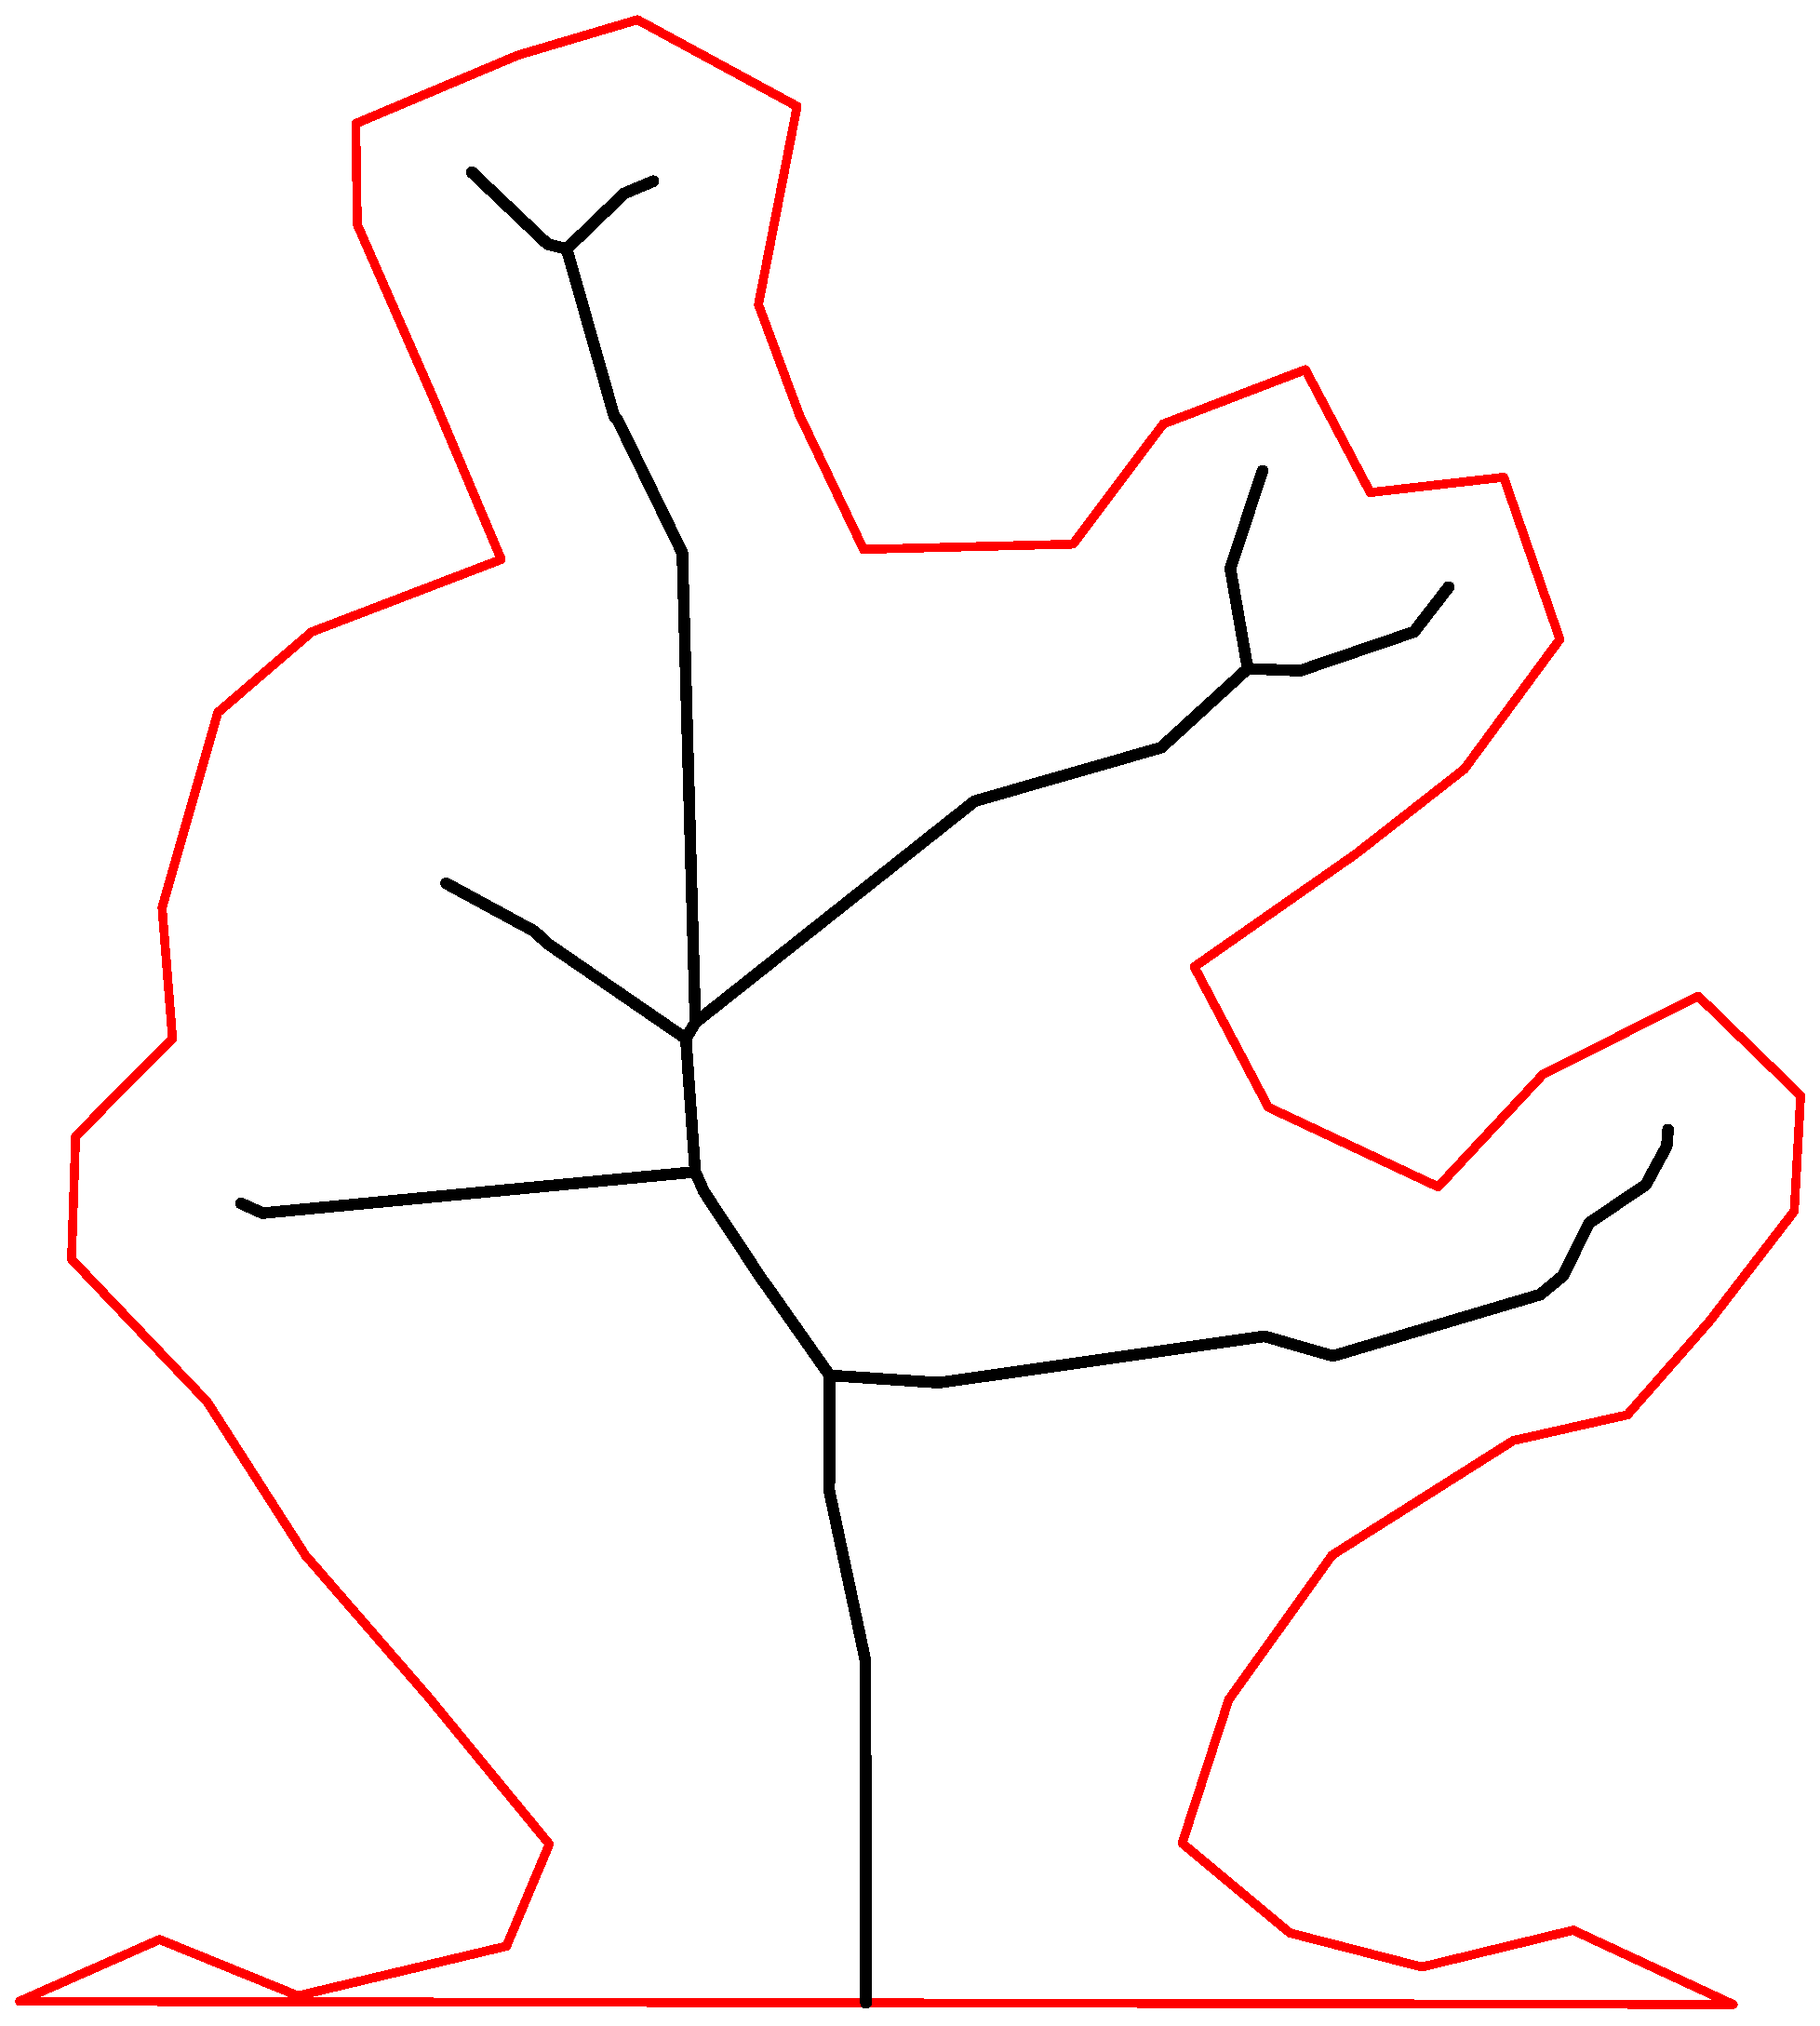
\includegraphics[width=0.4\textwidth]{Chapter4/Chapter4Figs/fig-skeleton.eps}
\caption{An example of polygon's skeleton.}
\label{fig-nhr-skeleton}
\end{figure}

Because this graph is calculated locally in each sensor node, node needs to know the location of only one point such that, if the packet is forwarded to that point, it still can find the way out the inner polygon by forwarding to the next point. We call such that point \textbf{endpoint}. On the other hand, from a point in the \emph{gateway}, we can re-construct the graph to find the way in from the gateway to the destination point. We call such that point \textbf{gate-point}. We also note that to reduce the node state, this graph is calculated only for each node to determine its \emph{endpoint}, and the nodes save the location of its \emph{endpoint} to its local memory, not the graph.
Algorithm \ref{algo-nhr-endpoint} describes how to construct such a skeleton and determine the \emph{endpoint} and \emph{gate-point} of a sensor node.

\begin{algorithm}[!htb]
\SetAlgoLined
\caption{Internal graph construction, endpoint and gate-point determination algorithm}
\label{algo-nhr-endpoint}
\Input{$N$: current sensor node}
\Output{$E_N$: endpoint of $N$\newline
$G_N$: gate-point of $N$}

\uIf{$N$ \emph{is not inside any inner polygons}} {
	$E_N \leftarrow N$\;
	$G_N \leftarrow null$\;
} 
\Else{
	$IP_{P_{hk}} \leftarrow$ inner polygon contains $N$\;
	$P_{h}P_{k} \leftarrow$ gateway of $IP_{P_{hk}}$\;
	$E_{IP_{P_{hk}}} \leftarrow$ set of edges of $IP_{P_{hk}}$\;
	$l \leftarrow$ perpendicular line from $N$ to $P_{h}P_{k}$\;
	$H \leftarrow l \cap P_{h}P_{k}$\;
	\uIf{$NH \cap \{E_{IP_{P_{hk}}} \setminus P_{h}P_{k}\} = \varnothing$}{
		$E_N \leftarrow H$\;
		$G_N \leftarrow null$\;
	}
	\Else {
		Construct Voronoi diagram $\upsilon$ of $IP_{P_{hk}}$\; 
		$\gamma \leftarrow$ Voronoi site contains $N$\;
		$V_j, V_{j+1}, ..., V_u \leftarrow$ Voronoi vertices of $\gamma$ inside $IP_{P_{hk}}$\;
		$K \leftarrow P_{i_h}P_{i_k} \cap e$ such that $e$ has a vertex inside $IP_{P_{hk}}$ and the other vertex outside $IP_{P_{hk}}$\;
		Eliminate all Voronoi edges not inside $IP_{P_{hk}}$ except $e$\;
		Construct graph from remaining edges\;
		Traversal the graph using BFS algorithm to find the shortest path from $V_j, V_{j+1}, ..., V_u$ to $K$\;
		$V_w\leftarrow$ is vertex corresponding to the shortest path among these paths\;
		$E_N \leftarrow V_w$\;
		$G_N \leftarrow K$\;
	}
}
\Return $E_N, G_N$\;
\end{algorithm}

By determining the \emph{endpoint} and \emph{gate-point} of a sensor node, we can route a packet to a destination node inside an inner polygon or route a packet from a source node inside an inner polygon to the outside of the convex hull. The details of this algorithm are presented in the next subsection. Note that this \emph{Internal Graph Construction} is performed only by nodes staying inside an inner polygon.

\subsection{Data Forwarding}
\label{data-forwarding}
In this subsection, we present the hole bypassing algorithm. As described above, the near hole routing path is constructed from VA-points. There are three type of VA-points: the source's VA-point, the VA-points which are vertices of scale octagon and the destination's VA-point. We use the octagon instead of the convex hull to reduce the number of VA-points' information stored in each packet, since the path constructed from the convex hull can contain a lot of VA-points and its number depends on the complexity of the convex hull. The routing path consists of three main periods: the first is from the source to its VA-point, the second is from the source's VA-point to the destination's VA-point and the last is from the destination's VA-point to the destination. Below we show how to determine these VA-points and the routing path of each period.

When a data packet is formed, the source node initiates its VA-point as its endpoint. The first period terminates immediately in case the source node is outside the convex hull. Otherwise, the packet is forwarded to this VA-point. At each intermediate node, the VA-point field is updated to the endpoint of current node. We note that the routing path inside the convex hull is different from each sensor node. It depends on the location of current sensor node, thus it still ensures the load balancing in inside the forbidden area. This period terminates when the packet reaches the \emph{gateway}. In case the source node does not belong to the \emph{near hole region}, it simply greedily forwards the packet the destination until it reaches an intermediate node belonging to the \emph{near hole region}.

Assume $I_s$ is this intermediate node. $I_s$ then uses its core polygon information $A$ to construct a scale polygon. This scale polygon is the image of core polygon $A$ through a homothetic transformation using a center $I$ chosen randomly inside the core polygon. The scale factor $\xi$ is computed based on the distance of $I_s$ to the convex hull and the system parameter $\delta$ as follows:\\
Let $d$ is maximum distance from $I$ to the vertices of $A$.
\begin{itemize}
\item $\xi = 1 + \frac{\delta \times R_c}{d}$ if $I_s$ is inside or on the edge of the convex hull
\item $\xi = 1 + \frac{d(C_P, I_s) \times R_c}{d}$ if $I_s$ is outside the convex hull 
\end{itemize}
$I_s$ also computes the destination's VA-point $I_d$ as follows:
\begin{itemize}
\item If the destination node $d$ is not inside any inner polygons, $I_d$ is the destination node.
\item Otherwise, $I_d$ is the \emph{gate-point} constructed from the internal graph of the inner polygon containing the destination node.
\end{itemize}

Then the algorithm \ref{algo-nhr-vap} is executed to determine VA-points which are vertices of scale octagon. Figure \ref{fig-nhr-vap} illustrates the algorithm.

\begin{figure}[!htb]
\centering
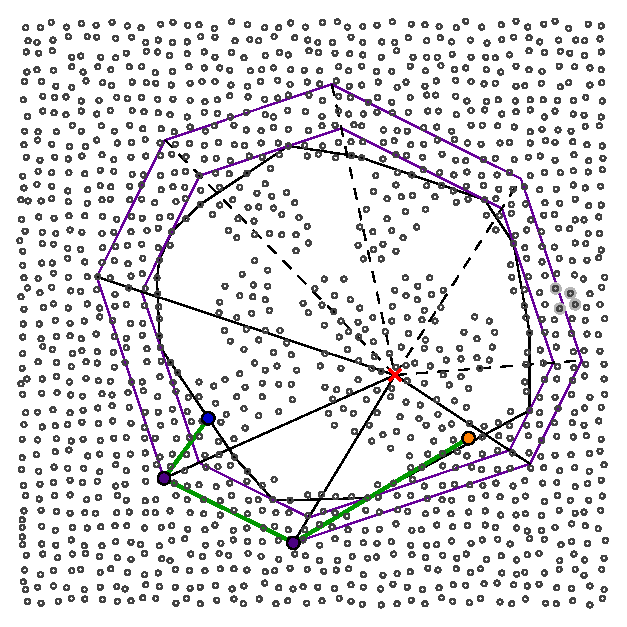
\includegraphics[width=0.4\textwidth]{Chapter4/Chapter4Figs/fig-octagon-vap.eps}
\caption{An example of choosing VA-points which are vertices of scale polygon.}
\label{fig-nhr-vap}
\end{figure}

\begin{algorithm}[!htb]
\SetAlgoLined
\caption{Virtual anchor points determination algorithm}
\label{algo-nhr-vap}
\nosemic Assume $I_s$ is current sensor node, $I_d$ is the destination's VA-point and $A' = \{A'_1, A'_2, ..., A'_m\}$ $(4 \leq m \leq 8)$ is the scale polygon with homothetic center $I$.\;
\nosemic Four points $L_s, L_d, R_s, R_d$ are computed as follows:\;
\uIf{$I_s$ is inside $A$}{
	$A'_i, A'_{i+1} \leftarrow$ two consecutive vertices of $A'$ such that $\bigtriangleup IA'_iA'_{i+1}$ contains $I_s$\;
	$L_s, R_s \leftarrow A'_i, A'_{i+1}$\;
}
\Else{
	$L_s, R_s \leftarrow$ view-limit vertices of $I_s$ respect to $A'$\;
}
\nosemic $L_d, R_d$ is computed same as $L_s, R_s$.\;
\nosemic Assume $L_s, L_s$ stay on the left side of $I_sI_d$ and $R_s, R_d$ stay on the right side of $I_sI_d$. The hole bypassing routing path is chosen as the shorter path between $\overrightarrow{I_sL_s...L_dI_d}$ and $\overrightarrow{I_sR_s...R_dI_d}$.
\end{algorithm}
The information of virtual anchor points is added to the packet header. The packet then is forwarded greedily to each virtual anchor point. 

In the last virtual anchor point, i.e. the destination's VA-point, it re-construct the internal graph of the inner polygon containing the destination in case the destination is inside an inner polygon, or it simply use the greedy protocol to forward the packet to the destination. If the destination is inside an inner polygon, the internal graph construction is performed in some specific nodes, that are the Voronoi vertices of the graph, not all the nodes in the routing path. In this process, the BFS algorithm is executed to trace back the shortest path from the \emph{gate-point} to the destination node. This process terminates when the packet reaches the \emph{endpoint} of the destination node.

Algorithm \ref{algo-nhr} presents the hole bypassing protocol.

\begin{algorithm}[!htb]
\SetAlgoLined
\caption{Hole bypassing protocol.}
\label{algo-nhr}
\Input{$N$: current sensor node\newline
$D$: destination node\newline
$AP$: the set of virtual anchor points\newline
$i$: current index of $AP$}
\Output{$next$: the location of the next hop}
Assume $getNextHopByGreedy(N, D$ returns the neighbor of $N$ which is nearest to $D$\;
$period \leftarrow$ current routing period\;
\If{$period = 1$}{
	$I_d \leftarrow$ endpoint of $N$\;
	$AP[6] \leftarrow I_d$\;
	$i \leftarrow 6$\;
}
\uIf{$N$ is a virtual anchor point}{
	$i \leftarrow i -1$\;
}
\ElseIf{$N$ is its endpoint}{
	$A \leftarrow$ core polygon\;
	$A' \leftarrow$ scale polygon\;
	$A'_1, A'_2, A'_3, A'_4 \leftarrow$ virtual anchor points computed from $A'$\;
	$AP[2..5] \leftarrow A'_1, A'_2, A'_3, A'_4$\;
	$i \leftarrow 5$\;
	% $I_s \leftarrow$ 
}
$next \leftarrow getNextHopByGreedy(N, AP[i])$\;
\Return $next$\;
\end{algorithm}

\section{Theoretical Analysis}
% \subsection{Validity of the protocol}
\subsection{Impact of parameter $\delta$ over the protocol}
The value of $\delta$ decides the area of the near hole region. The greater the value of $\delta$ is, the bigger the near hole region is. In the following, We show that the area of near hole region has a big impact on the two factors: energy consumption of the network and route stretch.

In case $\delta$ is big, the are of near hole region is big. Thus, the \emph{HPI} message is broadcast further, and more. Consequently, the energy consumption of the network increases. If $\delta$ is small, the \emph{HPI} message is broadcast lesser. Hence, the energy consumption of the network decreases.

In addition, if $\delta$ is small, the scale factor of the homothetic transformation is small. It makes all scale octagons almost the same. With a randomly deployed network, the density of sensor nodes is not really high, this would not create different routing path for different scale octagon. Thus, it decreases the load balancing. Vice versa, if $\delta$ is big, the scale factor is big, the virtual anchor points are far from the core polygon. It leads to the path enlargement problem.

According to mentioned analysis, obviously, the value of $\delta$ affects load balancing, energy consumption as well as route stretch. We also conducted experiments to prove these analysis and give a conclusion on the appropriate value of $\delta$.

\chapter{The WisSim toolkit}\label{chapter5}
The WisSim is a visual WIreless Sensor network SIMulation toolkit, which was developed by researchers at SEDIC Lab \cite{sedic} for building a software tool that could help researchers and algorithm designers to test their newly proposed algorithms for wireless sensor networks. 

The WiSSim architecture follows the Client-Server architecture where at the client side it provides the front-end components for the user to define the test networks, algorithms and execution scripts, and possibly ask for simulation then run the visualization and analysis tools to enjoy seeing the test analysis results provided with care towards the user convenience and deep understanding. At the back-end, it exploits a popular existing network simulator software, that is \emph{ns-2}. The WiSSim server acts as a connector to work with \emph{ns-2}: preparing the Tcl scripts to be executed in \emph{ns-2} and retrieving and interpreting the trace files outputted from \emph{ns-2}. Besides WisSim server also implements into the \emph{ns-2} core certain selected routing protocols \cite{sedic}.

The remaining of this chapter describes an overview of \emph{ns-2} simulator and some features which have been implemented in WisSim client by the author.

\section{ns-2 simulator overview}
The \emph{ns-2} is a discrete-event simulation framework, which was developed by researchers at UC Berkeley from 1995. The general architecture of \emph{ns-2} is presented in figure \ref{fig-ns2-arch}. 
\begin{figure}[!htb]
\centering
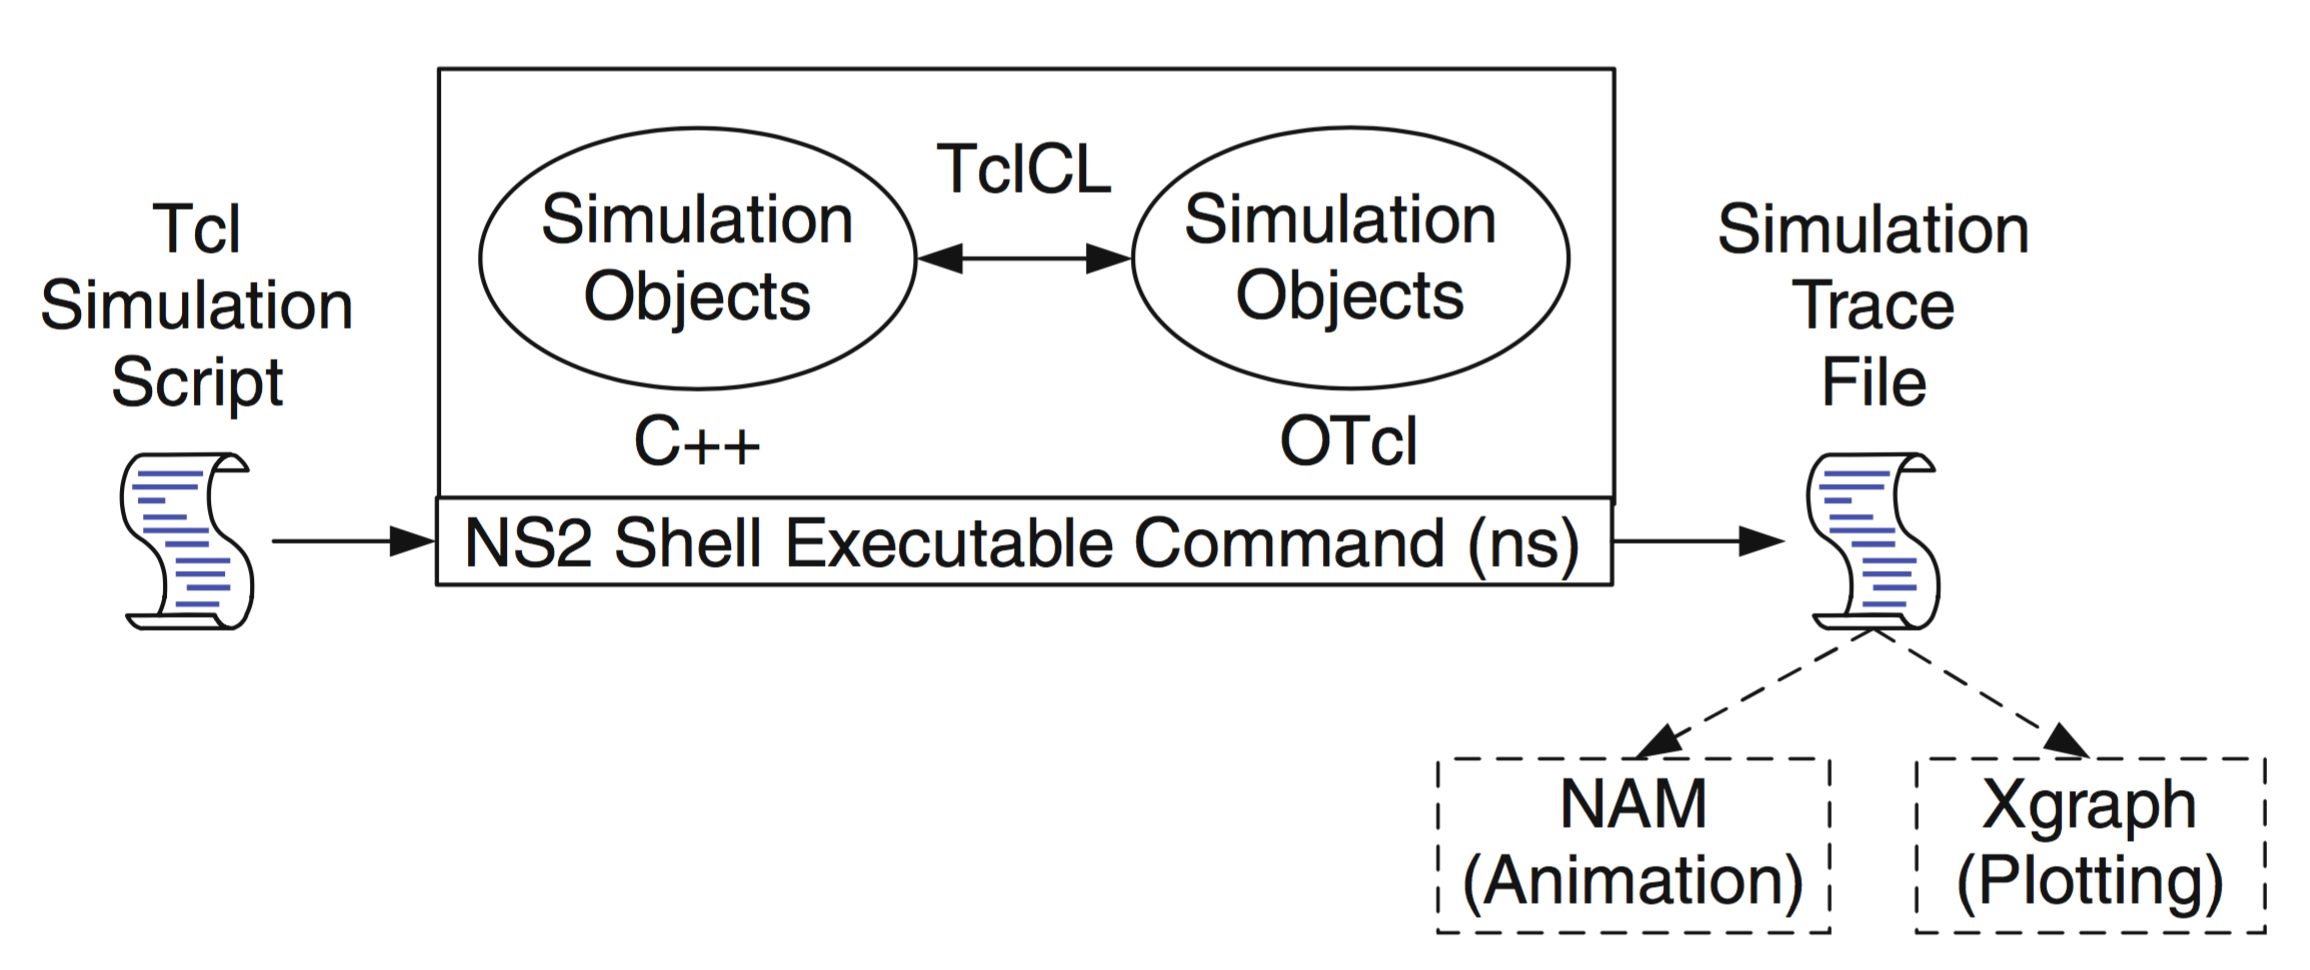
\includegraphics[width=0.6\textwidth]{Chapter5/Chapter5Figs/fig-ns2-arch.png}
\caption{The architecture of \emph{ns-2}.}
\label{fig-ns2-arch}
\end{figure} 

The simulation script is written in Tcl language. A simulation script must have:
\begin{itemize}
\item Network topology including network's size, number of sensor nodes, the configuration of each sensor nodes, network infrastructure, network protocol, and simulation time.
\item Declaration of events: the start time of the event, type of events, events' commands ...
\item Output format.
\end{itemize}
The output of simulation process called trace files. By analyzing these trace files, we can calculate network's metrics such as energy consumption, drop ratio or average path length, ...

The \emph{ns-2} uses two programming language: Tcl and C++. All the routing algorithms which are deployed into \emph{ns-2} core must be written in C++. The component of \emph{ns-2} could be classified into 4 groups based on their principal functions:
\begin{itemize}
\item Simulation-related Objects: controls and manages the simulation time. These objects are events, handlers, scheduler and simulator.
\item Network Objects: manages packet (transmit, receive, or drop).
\item Packet-related Objects: includes supporting packets.
\item Helper Objects: such as a routing protocol.
\end{itemize} 
As mentioned above, the \emph{ns-2} is a discrete-event simulation framework. More particularly, each event contains the time it will execute, its tasks and the link to the next event. These events create an event-chain, that is a single linked list and is created during the simulation process. Figure \ref{fig-ns2-event} shows an example of event-chain. 
\begin{figure}[!htb]
\centering
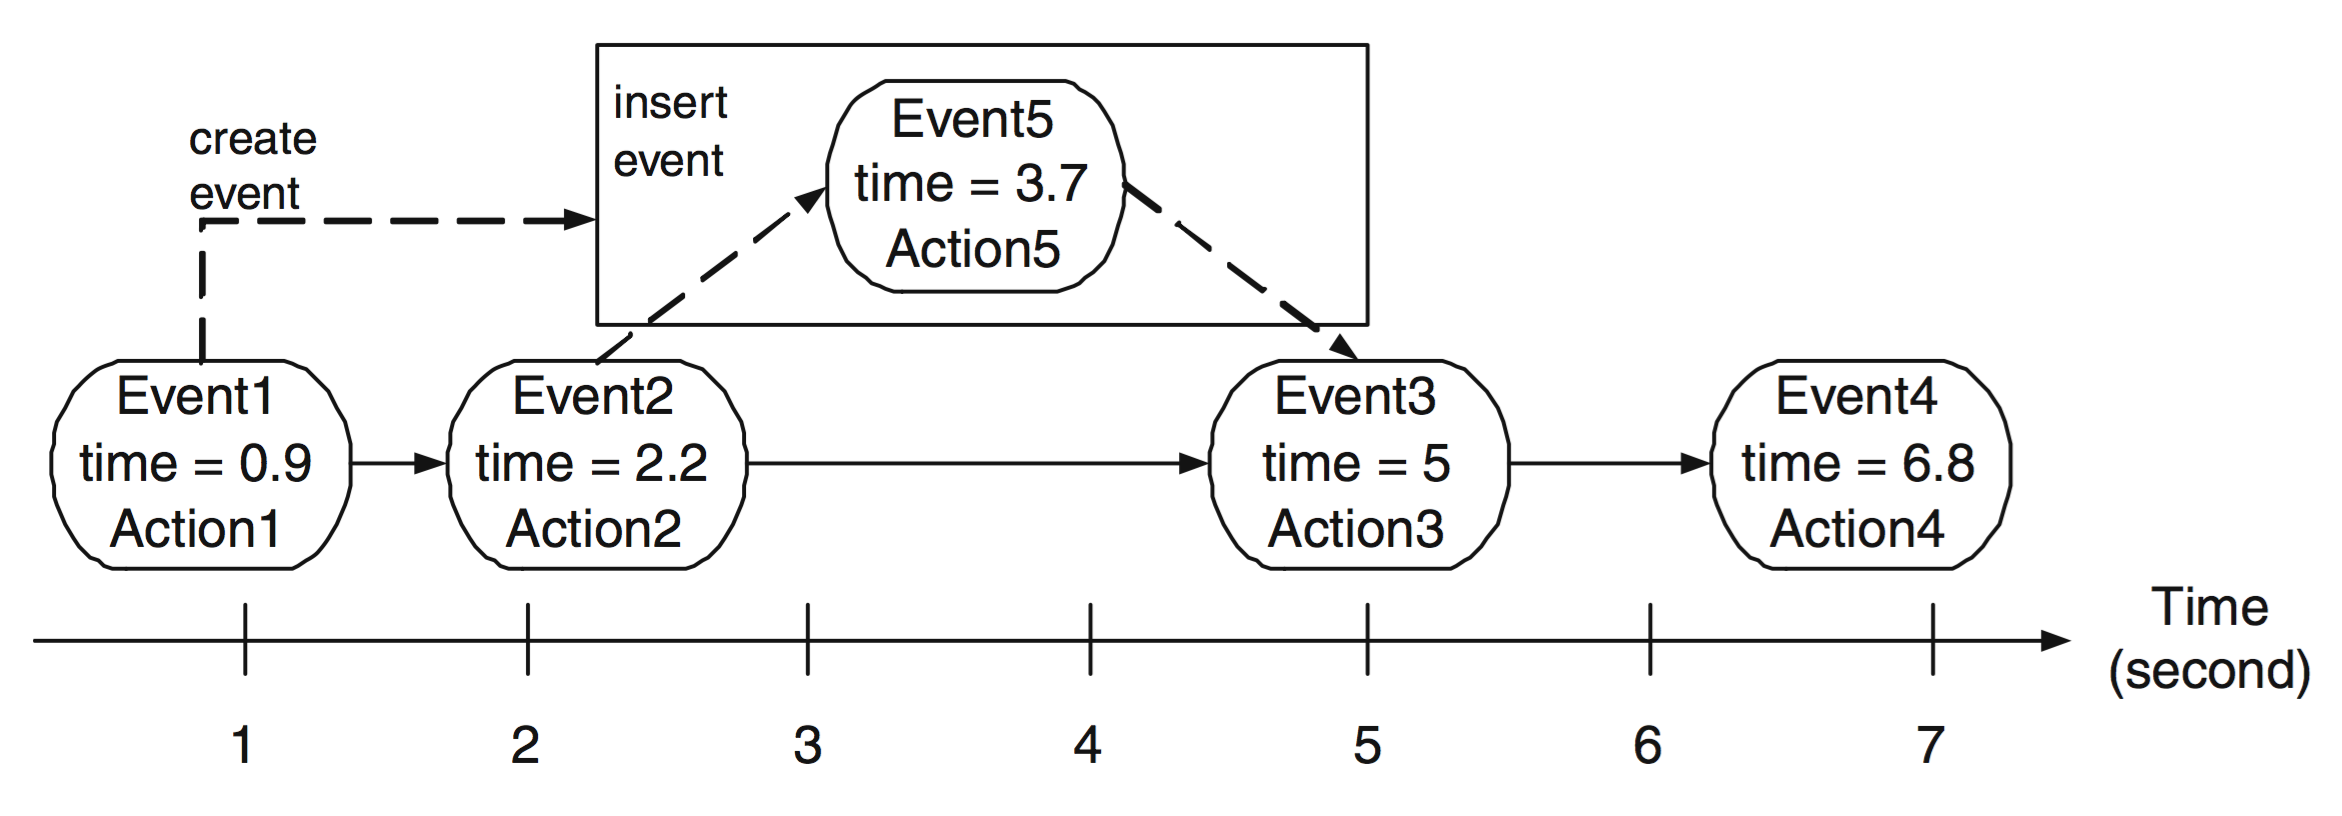
\includegraphics[width=0.6\textwidth]{Chapter5/Chapter5Figs/fig-ns2-event.png}
\caption{An example of event-chain in \emph{ns-2}.}
\label{fig-ns2-event}
\end{figure}

\section{WisSim Client}
\emph{WisSim} client is a software in the \emph{WisSim} toolkit which targets to have users create a network topology and analyze its properties. WisSim client consists of three main feature: WisSim Editor, WisSim Visualizer and WisSim Analyzer. In this section, we describe our addition features and improvements for WisSim client software. 
\subsection{Functional requirements}
\begin{table}[!htb]
\centering
\caption{Functional requirements}
\label{table-function-require}
\begin{tabular}{|p{2cm}|p{2cm}|p{2cm}|p{3cm}|p{2cm}|}
\cline{1-5}
Function        & Condition       & Input     & Output                                         & Module        \\ \cline{1-5}
Voronoi Diagram & Working project & Node list & Display                                        & WisSim Editor \\ \cline{1-5}
Graph           & Working project & Node list & Shortest path computed from Dijkstra algorithm & WisSim Editor \\ \cline{1-5}
\end{tabular}
\end{table}
\subsection{Class design}

\begin{table}[!htb]
\centering
\caption{Packet list.}
\label{table-class-design}
\begin{tabular}{|l|p{8cm}|}
\hline
Packet               & Implementation                                                                                                                                           \\ \hline
Graph/VoronoiDiagram & This packet contains implementation of Voronoi diagram construction algorithm and computational geometry library (such as line, point, circle, parabola) \\ \hline
Graph/Graph          & This packet implements primitive graph algorithms such as BFS, Dijkstra, ...                                                                             \\ \hline
\end{tabular}
\end{table}

\subsection{Screen design}
\begin{figure}[!htb]
\centering
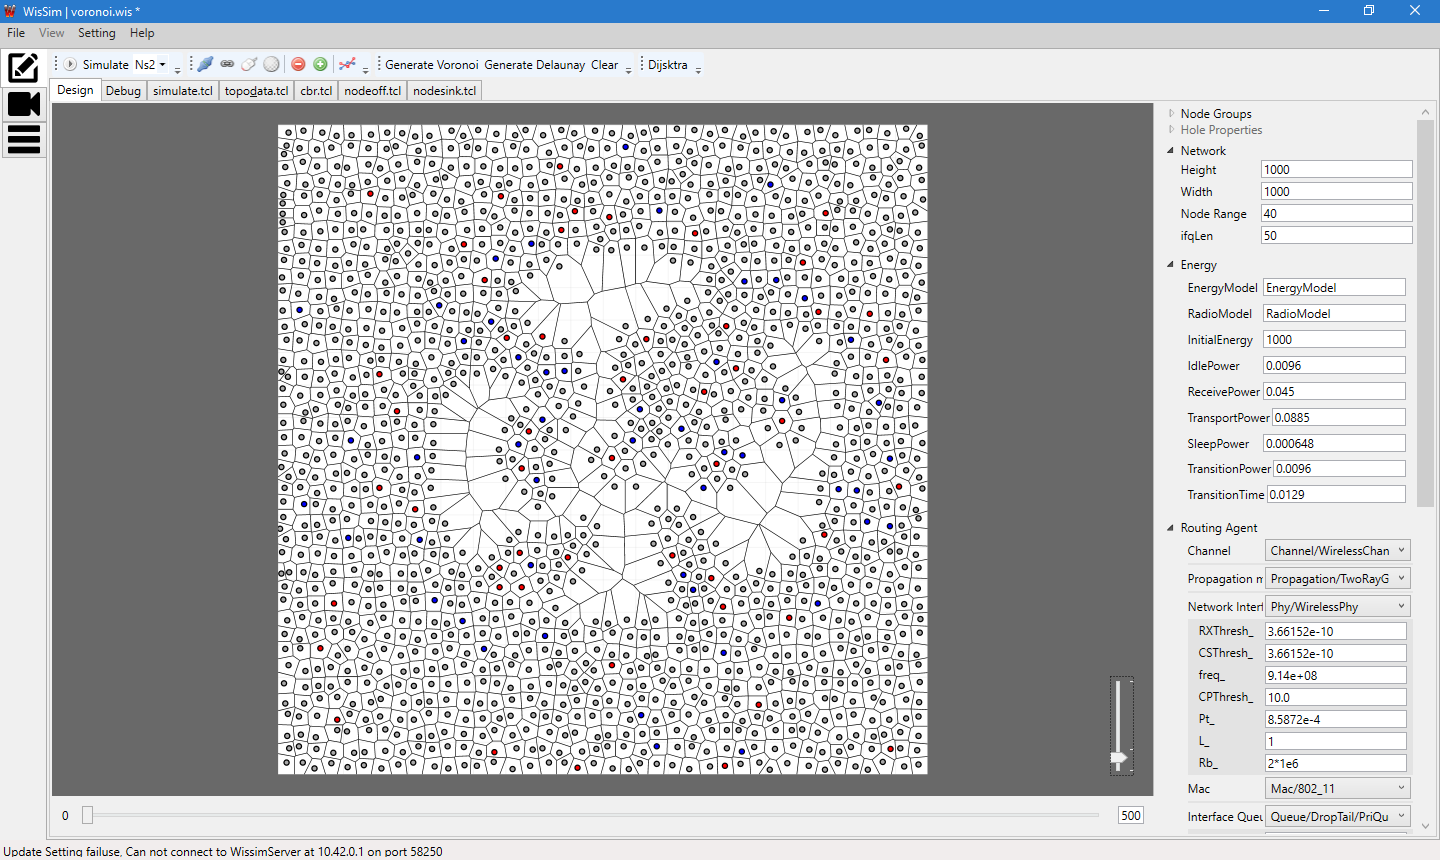
\includegraphics[width=0.8\textwidth]{Chapter5/Chapter5Figs/wissim-voronoi.png}
\caption{Screen of Voronoi diagram construction.}
\end{figure}

\begin{figure}[!htb]
\centering
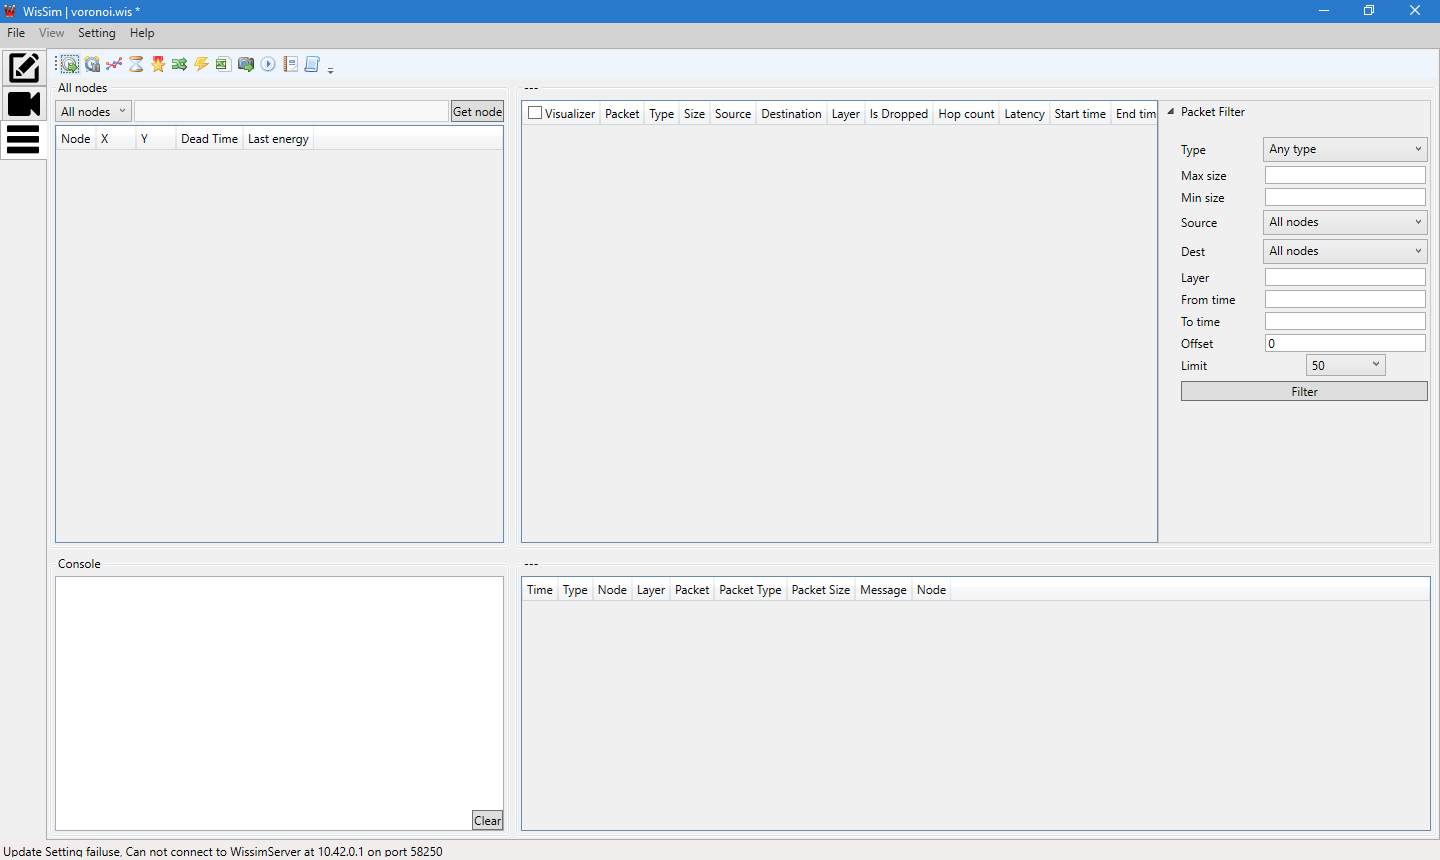
\includegraphics[width=0.8\textwidth]{Chapter5/Chapter5Figs/wissim-analyzer.png}
\caption{New design of WisSim Analyzer screen.}
\end{figure}
\chapter{Protocol implementation}\label{chapter6}
\section{Implementation details}
The proposed protocol is implemented in C++ and embedded into the core of current \emph{WisSim} toolkit. The source code is organized as follows.
\begin{itemize}
\item \emph{geometry}: contains implementation of geometry objects such as Point, Line, Circle, Vector, Parabola and its operators.
\item \emph{graph/voronoi}: contains implementation of Voronoi diagram construction using \emph{Fortune} algorithm.
\item \emph{nearholerouting}: contains implementation of the proposed protocol.
\subitem $-$\emph{nhr.cc}: definition of class \emph{NHRAgent}. This class is the core of the protocol.
\subitem $-$\emph{nhr.h}: header of class \emph{NHRAgent}.
\subitem $-$\emph{nhr\_graph.cc}: definition of class \emph{NHRGraph}. This class implements operators to construct the internal graph and compute the shortest path.
\subitem $-$\emph{nhr.cc}: header of class \emph{NHRGraph}.
\subitem $-$\emph{nhr\_packet.h}: declaration of packet header of protocol.
\subitem $-$\emph{nhr\_packet\_data.cc}: definition of class \emph{NHRPacketData}. This class provides methods to work with the packet payload such as add, remove, count, get size operator.
\subitem $-$\emph{nhr\_packet\_data.h}: header of class \emph{NHRPacketData}.
\end{itemize}

In order to integrate our routing protocol into \emph{ns-2} core, we defined a new packet type for our proposed protocol and gave default values for binded attributes.
Firstly, we added new \emph{NHR} packet type into \emph{tcl/lib/ns-packet.tcl}. We also added \emph{PT\_NHR} to the \emph{packet\_t} enumeration in \emph{common/packet.h}. Default values for binded attributes are given inside \emph{tcl/lib/ns-default.tcl}. Finally, we modified \emph{tcl/lib/ns-lib.tcl} to add procedures for creating a node with \emph{NHR} protocol.

In \emph{nhr.cc}, we implemented the core of our proposed protocol. The class \emph{NHRAgent} inherits class \emph{Agent} of \emph{ns-2} and overrides \emph{command()} and \emph{recv()} method.

\section{Source code listing}
\paragraph{Packet header \\}
The packet header of our proposed protocol is defined in \emph{nhr\_packet.h} source file. 
\begin{lstlisting}[language=C]{nhr_packet.h}
struct hdr_nhr {
    nsaddr_t daddr_;
    Point dest_;
    Point anchor_points[10];
    uint8_t ap_index;
    uint8_t type;

    inline int size() {
        return 11 * sizeof(Point) + 2 * sizeof(uint8_t) + sizeof(nsaddr_t);
    }

    static int offset_;

    inline static int &offset() {
        return offset_;
    }

    inline static struct hdr_nhr *access(const Packet *p) {
        return (struct hdr_nhr *) p->access(offset_);
    }
};
\end{lstlisting}

The meaning of each field is described below:
\begin{itemize}
\item \emph{daddr\_}: destination node' ID
\item \emph{dest\_}: destination node's location information
\item \emph{anchor\_points}: array of virtual anchor points
\item \emph{ap\_index}: current index of \emph{anchor\_points} array
\item \emph{type\_}: packet type. It receives one of following values:
\begin{itemize}
\item \emph{NHR\_CBR\_GPSR}: indicates greedy forwarding mode
\item \emph{NHR\_CBR\_AWARE\_SOURCE\_ESCAPE}: indicates near hole routing mode, from inner polygon to outside
\item \emph{NHR\_CBR\_AWARE\_SOURCE\_PIVOT}: indicates near hole routing mode
\item \emph{NHR\_CBR\_AWARE\_OCTAGON}: indicates near hole routing mode using scale octagon
\item \emph{NHR\_CBR\_AWARE\_DESTINATION}: indicates near hole routing mode for routing to destination
\end{itemize}
\end{itemize}
The \emph{size()} function returns the total size in byte of all above fields.

\paragraph{Core protocol \\}
Our core protocol is implemented in \emph{nhr.cc} source file. In this file, the \emph{recvData()} method is source code of the hole bypassing protocol. 
\begin{lstlisting}[language=C]{nhr.cc}
void NHRAgent::recvData(Packet *p) {
  struct hdr_cmn *cmh = HDR_CMN(p);
  struct hdr_nhr *edh = HDR_NHR(p);
  node *nexthop = NULL;

  if (cmh->direction() == hdr_cmn::UP 
      && edh->daddr_ == my_id_) // up to destination
  {
    port_dmux_->recv(p, 0);
    return;
  }

  if (edh->type == NHR_CBR_GPSR && !hole_.empty()) {
    edh->type = NHR_CBR_AWARE_SOURCE_ESCAPE;
    edh->ap_index = 1;
    edh->anchor_points[edh->ap_index] = endpoint_;
  }

  nexthop = getNeighborByGreedy(
              edh->anchor_points[edh->ap_index]);
  if (nexthop == NULL) {
    switch (edh->type) {
      case NHR_CBR_AWARE_SOURCE_ESCAPE:
        edh->anchor_points[1] = endpoint_;
        if (isPivot_) {
          edh->type = NHR_CBR_AWARE_SOURCE_PIVOT;
        }
        nexthop = getNeighborByGreedy(
                    edh->anchor_points[edh->ap_index]);
        if (nexthop != NULL) break;
      case NHR_CBR_AWARE_SOURCE_PIVOT:
        if (determineOctagonAnchorPoints(p)) {
          edh->type = NHR_CBR_AWARE_OCTAGON;
        } else {
            edh->ap_index = 0;
            edh->type = NHR_CBR_AWARE_DESTINATION;
        }
        nexthop = getNeighborByGreedy(
                    edh->anchor_points[edh->ap_index]);
        if (nexthop != NULL) break;
      case NHR_CBR_AWARE_OCTAGON:
        while (edh->ap_index > 2 && nexthop == NULL) {
          --edh->ap_index;
          nexthop = getNeighborByGreedy(
                      edh->anchor_points[edh->ap_index]);
        }
        if (edh->ap_index == 2) {
          edh->ap_index = 0;
          edh->type = NHR_CBR_AWARE_DESTINATION;
        }
        nexthop = getNeighborByGreedy(
                    edh->anchor_points[edh->ap_index]);
        if (nexthop != NULL) break;
      case NHR_CBR_AWARE_DESTINATION:
        routeToDest(p);
        nexthop = getNeighborByGreedy(
                    edh->anchor_points[edh->ap_index]);
        break;
      default:
        drop(p, DROP_RTR_NO_ROUTE);
        return;
    }
  }

  if (nexthop == NULL) {
    drop(p, DROP_RTR_NO_ROUTE);
    return;
  } else {
      cmh->direction() = hdr_cmn::DOWN;
      cmh->addr_type() = NS_AF_INET;
      cmh->last_hop_ = my_id_;
      cmh->next_hop_ = nexthop->id_;
      send(p, 0);
  }
}
\end{lstlisting}

\paragraph{Tcl hooking \\}
The procedure to initiate our protocol is written in Tcl language in \emph{ns-lib.tcl} source file. This procedure first creates an instance of routing protocol (line \#3), then sets up the parameters for each sensor node (line \#4 - \#11). Our protocol receives 2 commands to start specific events. In the beginning of the simulation process (0.0 second), all the sensor nodes start the protocol and send the HELLO packet to collect their neighbors information (line \#12). Then at second 30.0, the \emph{BOUNDHOLE} algorithm is started (line \#13).
\begin{lstlisting}[language=tcl]{ns-lib.tcl}
# NHR
Simulator instproc create-nhr-agent { node } {
  set ragent [new Agent/NHR]
  set addr [$node node-addr]
  $ragent addr $addr
  $ragent node $node
  if [Simulator set mobile_ip_] {
    $ragent port-dmux [$node demux]
  }
  $node addr $addr
  $node set ragent_ $ragent
  $self at 0.0  "$ragent start"    ;# start updates
  $self at 30 "$ragent boundhole"
  return $ragent
}
\end{lstlisting}

The default binding attributes for the protocol is declared in \emph{ns-default.tcl} source file. Our protocols takes 4 parameters. The name and meaning of each parameter are described in table \ref{table-param}.
\begin{table}[!htb]
\centering
\caption{Protocol parameter}
\label{table-param}
\begin{tabular}{|l|p{8cm}|}
\hline
Parameter               & Meaning                                                    \\ \hline
limit\_boundhole\_hop\_ & Upper bound of vertices number of the hole polygon         \\ \hline
hello\_period\_         & Period time to send HELLO packet (0 to send one time only) \\ \hline
range\_                 & 40m                                                        \\ \hline
delta\_                 & value of $\delta$ parameter                                \\ \hline
n\_                     & value of $\eta$ parameter                                  \\ \hline
\end{tabular}
\end{table}

\begin{lstlisting}[language=tcl]{ns-default.tcl}
Agent/NHR set limit_boundhole_hop_ 100
Agent/NHR set hello_period_ 0
Agent/NHR set range_ 40
Agent/NHR set delta_ 2.1
Agent/NHR set n_ 10
\end{lstlisting}
\chapter{Evaluation}\label{chapter7}
In this chapter, we compare our proposal (called NHR) with two existing proposals, GPSR \cite{gpsr}, BOUNDHOLE \cite{boundhole}. The metrics considered in our evaluation are the average energy consumption, the deviation of energy consumption, the energy consumption of individual sensor nodes, the network lifetime, the average path length and the routing path stretch. We assume that 1500 sensor nodes with 802.11 MAC protocol are deployed randomly in an area of 1000m x 1000m.

All parameters are summarized in table \ref{table-node-config}. Nodes follow the energy model suggested by \cite{energymodel} (see table \ref{table-node-energy}). We investigate the cases until the operation of a network reaches 1000s and a time when the first node fails (denoted by FNF).

\begin{table}[!htb]
\centering
\caption{Simulation parameters.}
\label{table-node-config}
\begin{tabular}{|l|l|}
\hline
Parameter                & Value              \\ \hline
Area                     & 1000m $\times$ 1000m \\ \hline
Number of nodes          & 1500               \\ \hline
Node communication range & 40m                \\ \hline
Number of CBR source     & 20/25/30/35/40/50  \\ \hline
Bandwidth                & 2Mbps              \\ \hline
Packet sending period    & 3s                 \\ \hline
Data packet size         & 50 bytes           \\ \hline
\end{tabular}
\end{table}

\begin{table}[!htb]
\centering
\caption{Node parameters.}
\label{table-node-energy}
\begin{tabular}{|l|l|}
\hline
Parameter                             & Value                    \\ \hline
Type of channel                       & Channel/WirelessChannel  \\ \hline
MAC type                              & MAC/802.11               \\ \hline
Network interface type                & Phy/WirelessPhy          \\ \hline
Interface queue model                 & Queue/DropTail/PriQueue  \\ \hline
Transmission of radio                 & Propagation/TwoRayGround \\ \hline
Energy model                          & EnergyModel              \\ \hline
Routing protocol                      & GPSR/BOUNDHOLE/NHR       \\ \hline
Node initial energy                   & 1000J/10J                \\ \hline
Length of the network interface queue & 50                       \\ \hline
Node idle power                       & 9.6mW                    \\ \hline
Node receive power                    & 45mW                     \\ \hline
Node transmit power                   & 88.5mW                   \\ \hline
\end{tabular}
\end{table}

\section{Average energy consumption}
The average energy consumption is calculated by dividing the total consumed energy of all the nodes to the number of the nodes. Figure \ref{fig-energy} plots the average energy consumption for six different routing protocols. It can be observed that the energy consumption for \emph{NHR} and the curve slope are smallest.
\begin{figure}[!htb]
  \centering
  \captionsetup{justification=centering}
  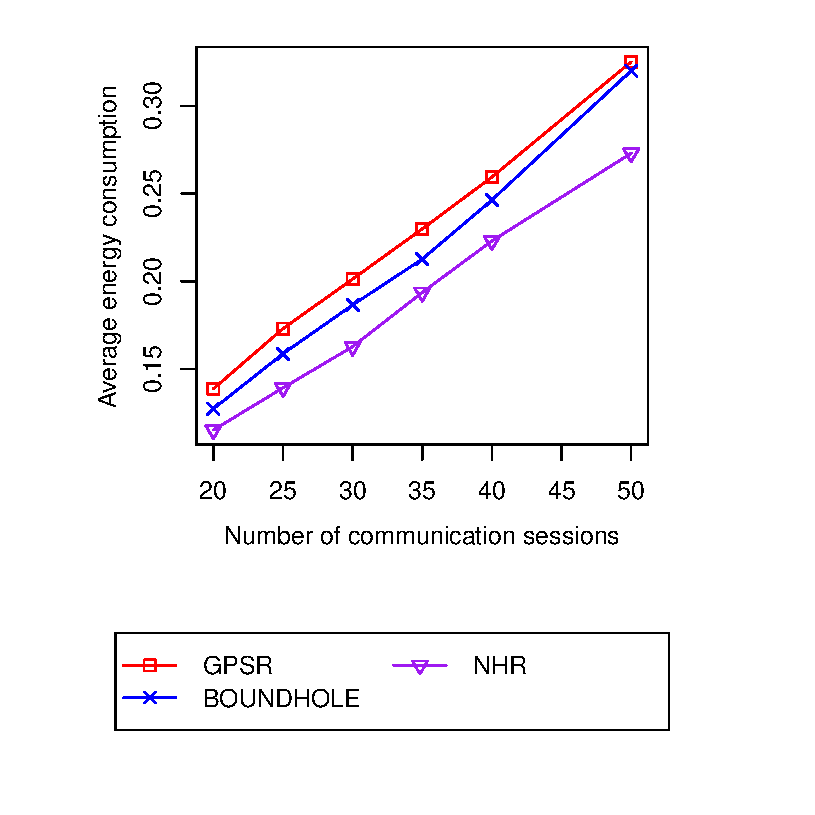
\includegraphics[width=0.6\textwidth]{Chapter7/Chapter7Figs/energy.eps}
\caption{Comparison of average energy consumption}
\label{fig-energy}
\end{figure}


\section{Deviation of energy consumption}
The deviation of energy consumption is calculated by the following formula: $\sigma = \sqrt{\frac{1}{K}\sum_{i=1}^{K}\left ( e_i - \frac{\sum_{i=1}^{K}e_i}{K} \right )^2}$, where $K$ is number of sensor nodes and $e_i$ is energy consumed by the $i^{th}$ node. The deviation of energy consumption of sensor nodes can give us a view of energy balancing. The more even the distribution of energy consumption is the better load balancing the protocol achieves. The smaller the deviation is, the higher the load balancing of network will be. 

\begin{figure}[!htb]
  \centering
  \captionsetup{justification=centering}
  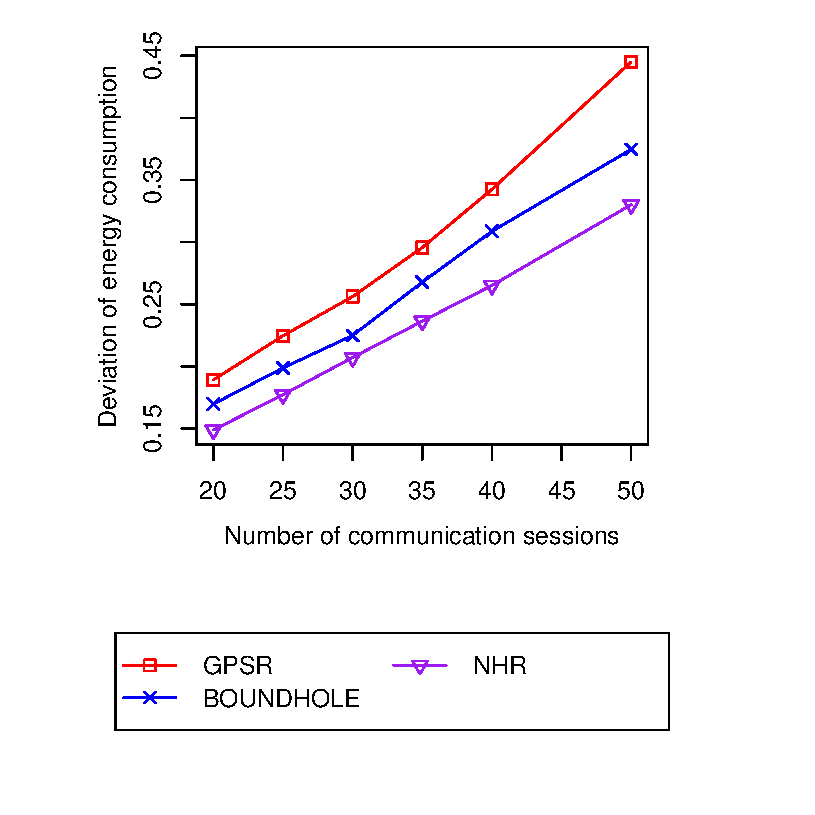
\includegraphics[width=0.6\textwidth]{Chapter7/Chapter7Figs/dev.eps}
\caption{Comparison of deviation of energy consumption}
\end{figure}

\section{Energy consumption of individual sensor nodes}
Figure \ref{fig-3d} scatters the energy consumption of individual sensor nodes in 3-dimension graphs. These figures give us a visual view of load balancing status of network. It is clear that, the per-node energy consumption by using GPSR and BOUNDHOLE are the most imbalanced. This imbalance is illustrated best by a look at the peaks at the center of figure \ref{fig-3d-gpsr}, \ref{fig-3d-boundhole}. The position of the peaks correspond to the location of the hole.
\begin{figure}[!htb]
\centering
\begin{subfigure}{0.5\textwidth}
  \centering
  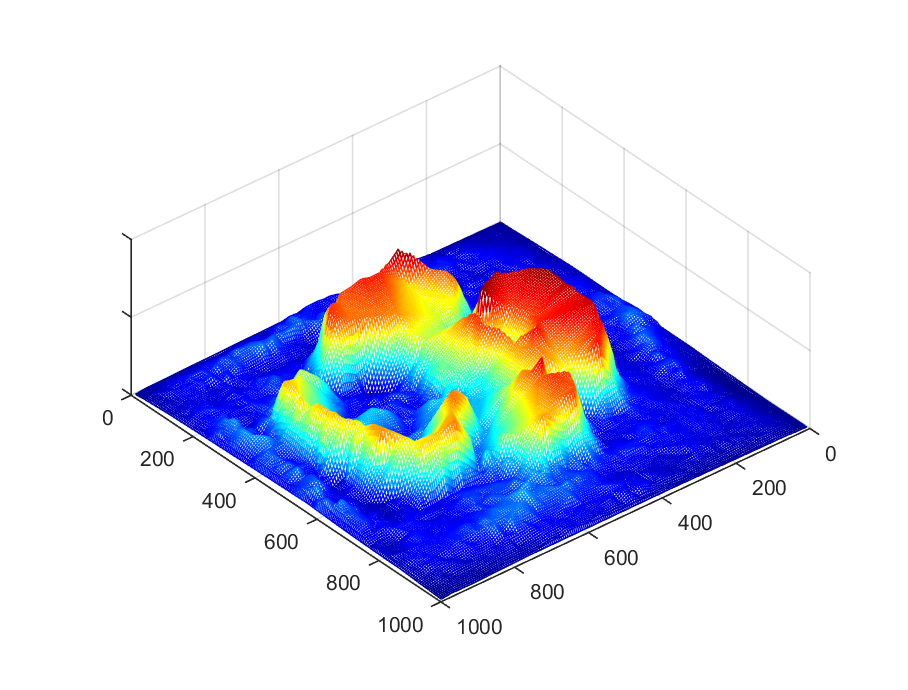
\includegraphics[width=0.8\textwidth]{Chapter7/Chapter7Figs/gpsr-energy.eps}
  \caption{GPSR}
  \label{fig-3d-gpsr}
\end{subfigure}%
\begin{subfigure}{0.5\textwidth}
  \centering
  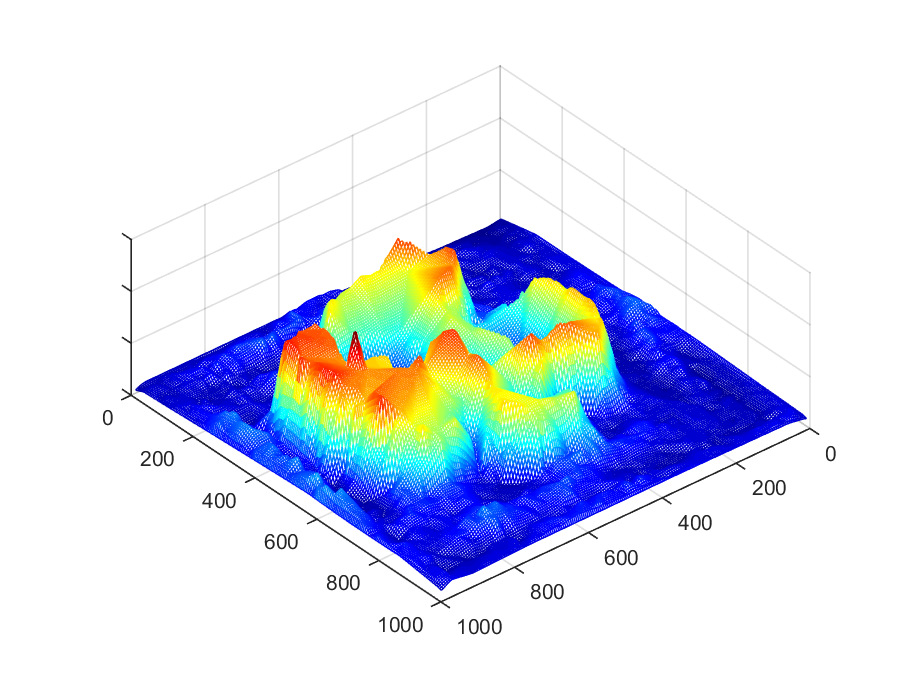
\includegraphics[width=0.8\textwidth]{Chapter7/Chapter7Figs/boundhole-energy.eps}
  \caption{BOUNDHOLE}
    \label{fig-3d-boundhole}
\end{subfigure}
\begin{subfigure}{0.5\textwidth}
  \centering
  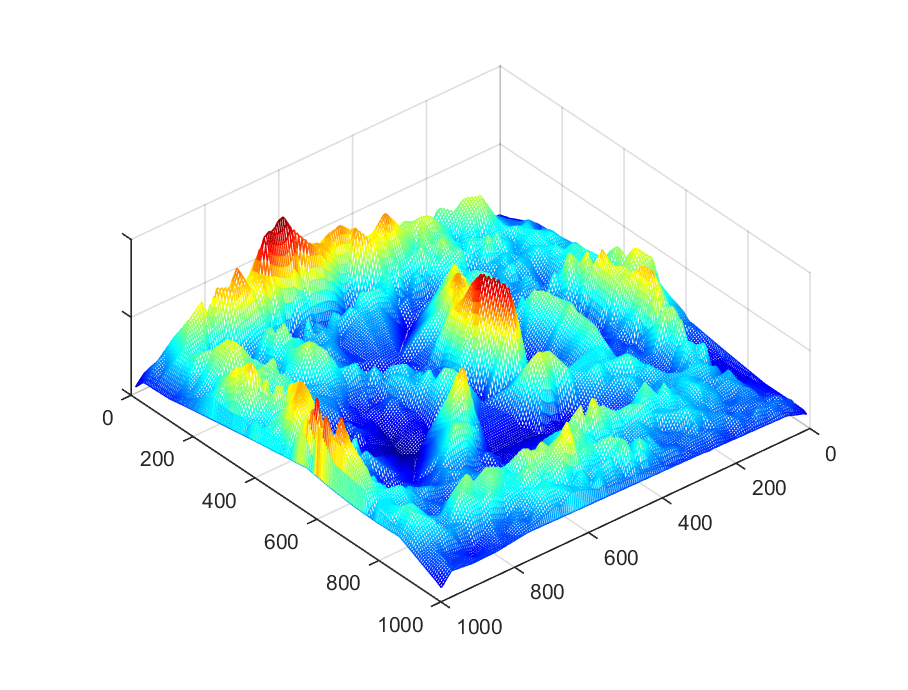
\includegraphics[width=0.8\textwidth]{Chapter7/Chapter7Figs/nhr-energy.eps}
  \caption{NHR}
\end{subfigure}
\caption{Visual view of energy consumption of individual sensor nodes}
\label{fig-3d}
\end{figure}

\section{Average path length}
The average path length is calculated as the average hop-count of all successfully transmitted packets. The comparison of the average path length for three protocols is shown in figure \ref{fig-path-length}.

\begin{figure}[!htb]
  \centering
  \captionsetup{justification=centering}
  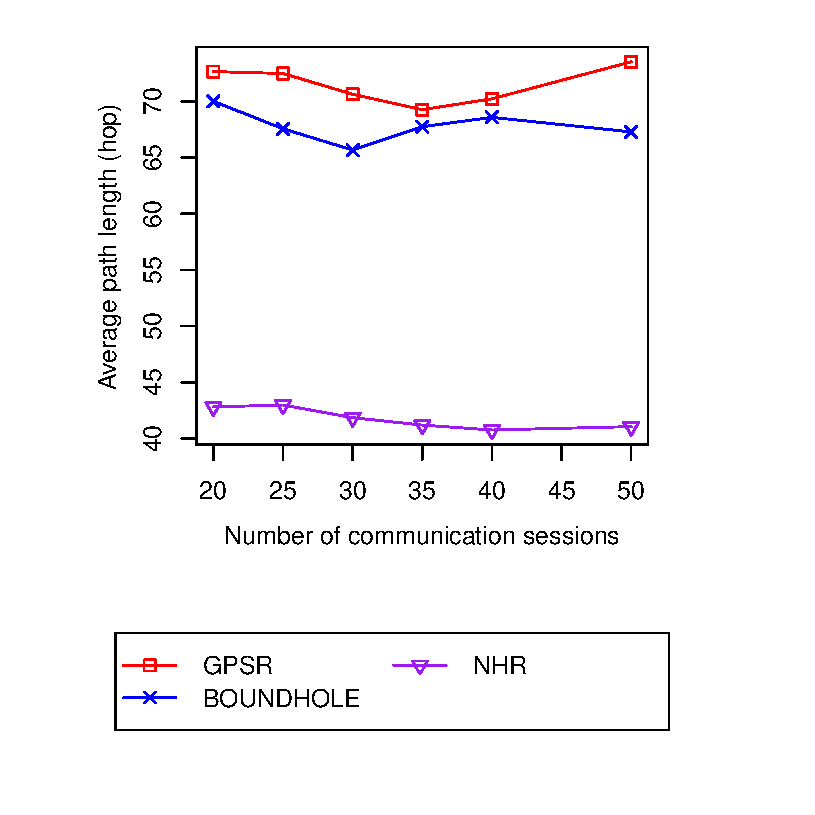
\includegraphics[width=0.6\textwidth]{Chapter7/Chapter7Figs/path.eps}
\caption{Comparison of average path length}
\label{fig-path-length}
\end{figure}

\section{Routing path stretch}
In this section we also evaluate the stretch by hop-count (i.e. the most practical stretch metric). The stretch by hop-count is the ratio between the hop-count of the routing path using routing protocol and the optimal path.

\section{Impact of $\delta$ on protocol}
We also conduct another experiment to investigate the impact of $\delta$ on the protocol. Three metrics are compared: the average path length, the average energy consumed, the deviation of energy consumption.

\begin{figure}[!htb]
\centering
\begin{subfigure}{0.5\textwidth}
  \centering
  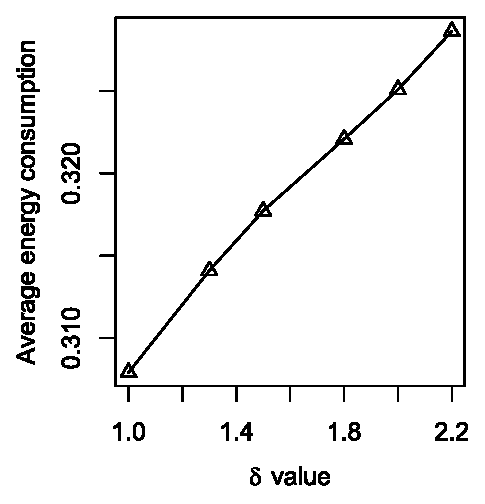
\includegraphics[width=0.8\textwidth]{Chapter7/Chapter7Figs/nhr-energy-plot.eps}
  \caption{Average energy consumption}
\end{subfigure}%
\begin{subfigure}{0.5\textwidth}
  \centering
  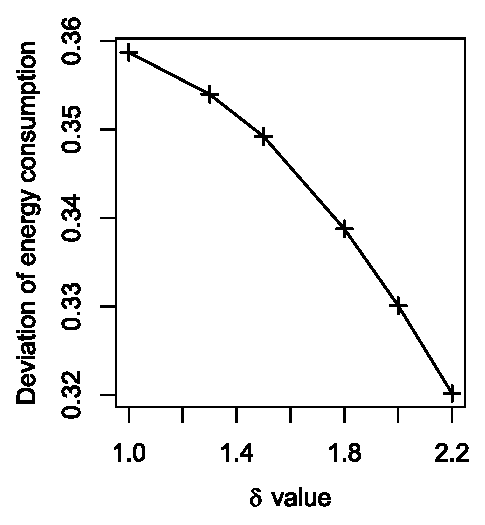
\includegraphics[width=0.8\textwidth]{Chapter7/Chapter7Figs/nhr-dev-plot.eps}
  \caption{Deviation of energy consumption}
\end{subfigure}
\begin{subfigure}{0.5\textwidth}
  \centering
  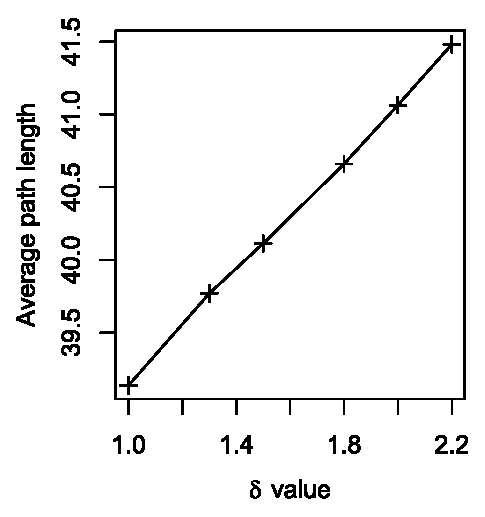
\includegraphics[width=0.8\textwidth]{Chapter7/Chapter7Figs/nhr-path-plot.eps}
  \caption{Average path length}
\end{subfigure}
\caption{Impact of $\delta$ on: average energy consumption, deviation of energy consumption and average path length}
\end{figure}

\chapter{Conclusion}\label{chapter8}
Routing protocol designing is classical problem in network communication. With the wireless sensor network, especially the wireless sensor network with harsh condition, the routing protocol designing becomes more difficult due to the existence of routing holes. Although a lot of protocols have been proposed, none of them targets and solves the near hole routing problem. In this thesis, we have thorough studied the routing in wireless sensor network with holes problem. Our research proposed a novel algorithm that targets and solves the near hole routing problem. Through theoretical analysis and simulations, we proved that our proposed ensures both two main requirements of a routing protocol: energy consumption and load balancing. As future work, we will extend our protocol for the multiple holes problem, support the network model with multiples sinks or propose an adaptive protocol for the dynamic routing hole.

\backmatter  
\appendix
%\chapter{TỔNG QUAN VỀ MÔ HÌNH MẠNG NƠRON} \label{Appendix1}
\section{Giới thiệu về mạng nơron nhân tạo }
\subsection{Định nghĩa}
Mạng nơron nhân tạo, Artificial Neural Network (ANN) gọi tắt là mạng nơron, neural network, là một mô hình xử lý thông tin phỏng theo cách thức xử lý thông tin của các hệ nơron sinh học. Nó được tạo lên từ một số lượng lớn các phần tử (gọi là phần tử xử lý hay nơron) kết nối với nhau thông qua các liên kết (gọi là trọng số liên kết) làm việc như một thể thống nhất để giải quyết một vấn đề cụ thể nào đó. 

Một mạng nơron nhân tạo được cấu hình cho một ứng dụng cụ thể (nhận dạng mẫu, phân loại dữ liệu, ...) thông qua một quá trình học từ tập các mẫu huấn luyện. Về bản chất học chính là quá trình hiệu chỉnh trọng số liên kết giữa các nơron.
\subsection{Lịch sử phát triển mạng nơron}
Các nghiên cứu về bộ não con người đã được tiến hành từ hàng nghìn năm nay. Cùng với sự phát triển của khoa học kĩ thuật đặc biệt là những tiến bộ trong ngành điện tử hiện đại, việc con người bắt đầu nghiên cứu các nơron nhân tạo là hoàn toàn tự nhiên. Sự kiện đầu tiên đánh dấu sự ra đời của mạng nơron nhân tạo diễn ra vào năm 1943 khi nhà thần kinh học Warren McCulloch và nhà toán học Walter Pitts viết bài báo mô tả cách thức các nơron hoạt động. Họ cũng đã tiến hành xây dựng một mạng nơron đơn giản bằng các mạch điện. Các nơron của họ được xem như là các thiết bị nhị phân với ngưỡng cố định. Kết quả của các mô hình này là các hàm logic đơn giản chẳng hạn như “ a OR b” hay “a AND b”. 

Tiếp bước các nghiên cứu này, năm 1949 Donald Hebb cho xuất bản cuốn sách Organization of Behavior. Cuốn sách đã chỉ ra rằng các nơron nhân tạo sẽ trở lên hiệu quả hơn sau mỗi lần chúng được sử dụng. 
Những tiến bộ của máy tính đầu những năm 1950 giúp cho việc mô hình hóa các nguyên lý của những lý thuyết liên quan tới cách thức con người suy nghĩ đã trở thành hiện thực. Nathanial Rochester sau nhiều năm làm việc tại các phòng thí nghiệm nghiên cứu của IBM đã có những nỗ lực đầu tiên để mô phỏng một mạng nơron. Trong thời kì này tính toán truyền thống đã đạt được những thành công rực rỡ trong khi đó những nghiên cứu về nơron còn ở giai đoạn sơ khai. Mặc dù vậy những người ủng hộ triết lý “thinking machines” (các máy biết suy nghĩ) vẫn tiếp tục bảo vệ cho lập trường của mình. 

Năm 1956 dự án Dartmouth nghiên cứu về trí tuệ nhân tạo (Artificial Intelligence) đã mở ra thời kỳ phát triển mới cả trong lĩnh vực trí tuệ nhân tạo lẫn mạng nơron. Tác động tích cực của nó là thúc đẩy hơn nữa sự quan tâm của các nhà khoa học về trí tuệ nhân tạo và quá trình xử lý ở mức đơn giản của mạng nơron trong bộ não con người. 
Những năm tiếp theo của dự án Dartmouth, John von Neumann đã đề xuất việc mô phỏng các nơron đơn giản bằng cách sử dụng rơle điện áp hoặc đèn chân không. Nhà sinh học chuyên nghiên cứu về nơron Frank Rosenblatt cũng bắt đầu nghiên cứu về Perceptron. Sau thời gian nghiên cứu này Perceptron đã được cài đặt trong phần cứng máy tính và được xem như là mạng nơron lâu đời nhất còn được sử dụng đến ngày nay. Perceptron một tầng rất hữu ích trong việc phân loại một tập các đầu vào có giá trị liên tục vào một trong hai lớp. Perceptron tính tổng có trọng số các đầu vào, rồi trừ tổng này cho một ngưỡng và cho ra một trong hai giá trị mong muốn có thể. Tuy nhiên Perceptron còn rất nhiều hạn chế, những hạn chế này đã được chỉ ra trong cuốn sách về Perceptron của Marvin Minsky và Seymour Papert viết năm 1969. 

Năm 1959, Bernard Widrow và Marcian Hoff thuộc trường đại học Stanford đã xây dựng mô hình ADALINE (ADAptive LINear Elements) và MADALINE. (Multiple ADAptive LINear Elements). Các mô hình này sử dụng quy tắc học Least-Mean-Squares (LMS: Tối thiểu bình phương trung bình). MADALINE là mạng nơron đầu tiên được áp dụng để giải quyết một bài toán thực tế. Nó là một bộ lọc thích ứng có khả năng loại bỏ tín hiệu dội lại trên đường dây điện thoại. Ngày nay mạng nơron này vẫn được sử dụng trong các ứng dụng thương mại. 

Năm 1974 Paul Werbos đã phát triển và ứng dụng phương pháp học lan truyền ngược ( back-propagation). Tuy nhiên phải mất một vài năm thì phương pháp này mới trở lên phổ biến. Các mạng lan truyền ngược được biết đến nhiều nhất và được áp dụng rộng dãi nhất nhất cho đến ngày nay. 

Thật không may, những thành công ban đầu này khiến cho con người nghĩ quá lên về khả năng của các mạng nơron. Chính sự cường điệu quá mức đã có những tác động không tốt đến sự phát triển của khoa học và kỹ thuật thời bấy giờ khi người ta lo sợ rằng đã đến lúc máy móc có thể làm mọi việc của con người. Những lo lắng này khiến người ta bắt đầu phản đối các nghiên cứu về mạng neuron. Thời kì tạm lắng này kéo dài đến năm 1981. 

Năm 1982 trong bài báo gửi tới viện khoa học quốc gia, John Hopfield bằng sự phân tích toán học rõ ràng, mạch lạc, ông đã chỉ ra cách thức các mạng nơron làm việc và những công việc chúng có thể thực hiện được. Cống hiến của Hopfield không chỉ ở giá trị của những nghiên cứu khoa học mà còn ở sự thúc đẩy trở lại các nghiên cứu về mạng neuron. 
Cũng trong thời gian này, một hội nghị với sự tham gia của Hoa Kỳ và Nhật Bản bàn về việc hợp tác/cạnh tranh trong lĩnh vực mạng nơron đã được tổ chức tại Kyoto, Nhật Bản. Sau hội nghị, Nhật Bản đã công bố những nỗ lực của họ trong việc tạo ra máy tính thế hệ thứ 5. Tiếp nhận điều đó, các tạp chí định kỳ của Hoa Kỳ bày tỏ sự lo lắng rằng nước nhà có thể bị tụt hậu trong lĩnh vực này. Vì thế, ngay sau đó, Hoa Kỳ nhanh chóng huy động quĩ tài trợ cho các nghiên cứu và ứng dụng mạng neuron. 

Năm 1985, viện vật lý Hoa Kỳ bắt đầu tổ chức các cuộc họp hàng năm về mạng neuron ứng dụng trong tin học (Neural Networks for Computing). 
Năm 1987, hội thảo quốc tế đầu tiên về mạng neuron của Viện các kỹ sư điện và điện tử IEEE (Institute of Electrical and Electronic Engineer) đã thu hút hơn 1800 người tham gia. 

Ngày nay, không chỉ dừng lại ở mức nghiên cứu lý thuyết, các nghiên cứu ứng dụng mạng nơron để giải quyết các bài toán thực tế được diễn ra ở khắp mọi nơi. Các ứng dụng mạng nơron ra đời ngày càng nhiều và ngày càng hoàn thiện hơn. Điển hình là các ứng dụng: xử lý ngôn ngữ (Language Processing), nhận dạng kí tự (Character Recognition), nhận dạng tiếng nói (Voice Recognition), nhận dạng mẫu (Pattern Recognition), xử lý tín hiệu (Signal Processing), Lọc dữ liệu (Data Filtering),\ldots 

\subsection{So sánh mạng nơron với máy tính truyền thống}
Các mạng nơron có cách tiếp cận khác trong giải quyết vấn đề so với máy tính truyền thống. Các máy tính truyền thống sử dụng cách tiếp cận theo hướng giải thuật, tức là máy tính thực hiện một tập các chỉ lệnh để giải quyết một vấn đề. Vấn đề được giải quyết phải được biết và phát biểu dưới dạng một tập chỉ lệnh không nhập nhằng. Những chỉ lệnh này sau đó phải được chuyển sang một chương trình ngôn ngữ bậc cao và chuyển sang mã máy để máy tính có thể hiểu được. 
Trừ khi các bước cụ thể mà máy tính cần tuân theo được chỉ ra rõ ràng, máy tính sẽ không làm được gì cả. Điều đó giới hạn khả năng của các máy tính truyền thống ở phạm vi giải quyết các vấn đề mà chúng ta đã hiểu và biết chính xác cách thực hiện. Các máy tính sẽ trở lên hữu ích hơn nếu chúng có thể thực hiện được những việc mà bản thân con người không biết chính xác là phải làm như thế nào. 
Các mạng nơron xử lý thông tin theo cách thức giống như bộ não con người. Mạng được tạo nên từ một số lượng lớn các phần tử xử lý được kết nối với nhau làm việc song song để giải quyết một vấn đề cụ thể. Các mạng nơron học theo mô hình, chúng không thể được lập trình để thực hiện một nhiệm vụ cụ thể. Các mẫu phải được chọn lựa cẩn thận nếu không sẽ rất mất thời gian, thậm chí mạng sẽ hoạt động không đúng. Điều hạn chế này là bởi vì mạng tự tìm ra cách giải quyết vấn đề, thao tác của nó không thể dự đoán được. 
Các mạng nơron và các máy tính truyền thống không cạnh tranh nhau mà bổ sung cho nhau. Có những nhiệm vụ thích hợp hơn với máy tính truyền thống, ngược lại có những nhiệm vụ lại thích hợp hơn với các mạng nơron. Thậm chí rất nhiều nhiệm vụ đòi hỏi các hệ thống sử dụng tổ hợp cả hai cách tiếp cận để thực hiện được hiệu quả cao nhất. (thông thường một máy tính truyền thống được sử dụng để giám sát mạng nơron)

\section{Nơron sinh học và nơron nhân tạo}
\subsection{Nơron sinh học}
Qua quá trình nghiên cứu về bộ não, người ta thấy rằng: bộ não con người bao gồm khoảng 1011 nơron tham gia vào khoảng 1015 kết nối trên các đường truyền. Mỗi đường truyền này dài khoảng hơn một mét. Các nơron có nhiều đặc điểm chung với các tế bào khác trong cơ thể, ngoài ra chúng còn có những khả năng mà các tế bào khác không có được, đó là khả năng nhận, xử lý và truyền các tín hiệu điện hóa trên các đường mòn nơron, các con đường này tạo nên hệ thống giao tiếp của bộ não.

Mỗi nơron sinh học có 3 thành phần cơ bản: 
\begin{itemize}
\item Các nhánh vào hình cây ( dendrites) 
\item Thân tế bào (cell body) 
\item Sợi trục ra (axon) 
\end{itemize}

Các nhánh hình cây truyền tín hiệu vào đến thân tế bào. Thân tế bào tổng hợp và xử lý cho tín hiệu đi ra. Sợi trục truyền tín hiệu ra từ thân tế bào này sang nơron khác. Điểm liên kết giữa sợi trục của nơron này với nhánh hình cây của nơron khác gọi là synapse. Liên kết giữa các nơron và độ nhạy của mỗi synapse được xác định bởi quá trình hóa học phức tạp. Một số cấu trúc của nơron được xác định trước lúc sinh ra. Một số cấu trúc được phát triển thông qua quá trình học. Trong cuộc đời cá thể, một số liên kết mới được hình thành, một số khác bị hủy bỏ. 

Như vậy nơron sinh học hoạt động theo cách thức sau: nhận tín hiệu đầu vào, xử lý các tín hiệu này và cho ra một tín hiệu output. Tín hiệu output này sau đó được truyền đi làm tín hiệu đầu vào cho các nơron khác.

Dựa trên những hiểu biết về nơron sinh học, con người xây dựng nơron nhân tạo với hy vọng tạo nên một mô hình có sức mạnh như bộ não.

\subsection{Nơron nhân tạo}
Một nơron là một đơn vị xử lý thông tin và là thành phần cơ bản của một mạng nơron. Cấu trúc của một nơron được mô tả trên hình \ref{neuralnhantao}: 
\begin{figure}[!htbp] 
  \begin{center}
    %\leavevmode
    \ifpdf
      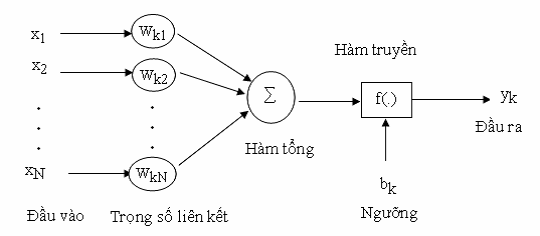
\includegraphics[scale=1.0]{Appendix1/nerualnhantao}
    \else
      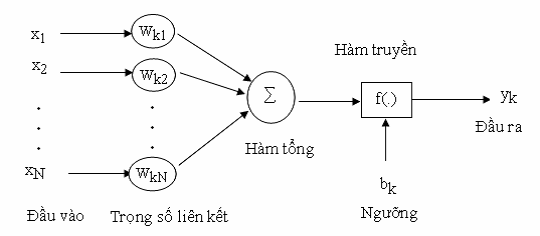
\includegraphics[scale=1.0]{Appendix1/nerualnhantao}
    \fi
    \caption{Cấu trúc nơron nhân tạo}
    \label{neuralnhantao}
  \end{center}
\end{figure}

Các thành phần cơ bản của một nơron nhân tạo bao gồm: 
\begin{itemize}
\item \textbf{Tập các đầu vào}: Là các tín hiệu vào (\textit{input signals}) của nơron, các tín hiệu này thường được đưa vào dưới dạng một vector N chiều. 
\item \textbf{Tập các liên kết}: Mỗi liên kết được thể hiện bởi một trọng số (gọi là trọng số liên kết – S\textit{ynaptic weight}). Trọng số liên kết giữa tín hiệu vào thứ j với nơron k thường được kí hiệu là wkj. Thông thường, các trọng số này được khởi tạo một cách ngẫu nhiên ở thời điểm khởi tạo mạng và được cập nhật liên tục trong quá trình học mạng. 
\item \textbf{Bộ tổng} (\textit{Summing function}): Thường dùng để tính tổng của tích các đầu vào với trọng số liên kết của nó. 
\item \textbf{Ngưỡng} (còn gọi là một độ lệch - \textit{bias}): Ngưỡng này thường được đưa vào như một thành phần của hàm truyền. 
\item \textbf{Hàm truyền} (\textit{Transfer function}) : Hàm này được dùng để giới hạn phạm vi đầu ra của mỗi nơron. Nó nhận đầu vào là kết quả của hàm tổng và ngưỡng đã cho. Thông thường, phạm vi đầu ra của mỗi nơron được giới hạn trong đoạn [0,1] hoặc [-1, 1]. Các hàm truyền rất đa dạng, có thể là các hàm tuyến tính hoặc phi tuyến. Việc lựa chọn hàm truyền nào là tuỳ thuộc vào từng bài toán và kinh nghiệm của người thiết kế mạng.
\item \textbf{Đầu ra}: Là tín hiệu đầu ra của một nơron, với mỗi nơron sẽ có tối đa là một đầu ra. 
\end{itemize}

\subsection{Kiến trúc mạng nơron}
Người ta chia mạng nơron làm hai kiến trúc: 
\begin{itemize}

\item \textbf{Kiến trúc truyền thẳng} (\textit{feedforward architechture}): là kiểu kiến trúc mạng không có các kết nối ngược trở lại từ các nơron đầu ra về các nơron đầu vào; mạng không lưu lại các giá trị output trước và các trạng thái kích hoạt của nơron. Các mạng nơron truyền thẳng cho phép tín hiệu di chuyển theo một đường duy nhất; từ đầu vào tới đầu ra, đầu ra của một tầng bất kì sẽ không ảnh hưởng tới tầng đó.
\item \textbf{Kiến trúc phản hồi} (\textit{Feedback architecture}): là kiểu kiến trúc mạng có các kết nối từ nơron đầu ra tới nơron đầu vào. Mạng lưu lại các trạng thái trước đó, và trạng thái tiếp theo không chỉ phụ thuộc vào các tín hiệu đầu vào mà còn phụ thuộc vào các trạng thái trước đó của mạng.
\end{itemize}
%\chapter{Phụ lục B}
Đây là phụ lục B 
% ------------------------------------------------------------------------

%%% Local Variables: 
%%% mode: latex
%%% TeX-master: "../thesis"
%%% End: 


\clearpage
\bibliographystyle{Classes/CUEDbiblio}
\renewcommand{\bibname}{References} % changes default name Bibliography to References
\bibliography{References} % References file

\end{document}
